\documentclass[twoside]{report}

\usepackage{Preamble}                 % Use preamble defined by me
\usetikzlibrary{quantikz}             % Package for drawing quantum circuits

\title{Time Simulation of an Anisotropic Heisenberg Chain in a Superconducting Quantum Processor with Qiskit}
\author{Diego Alejandro Herrera Rojas}
\date{\today}

\begin{document}
  \begin{titlepage}
  \begin{center}
    \vspace*{1cm}
    
\includegraphics[scale=0.1]{Images/EscudoUnal.png}\\
    \vspace*{1cm}
    \huge
    \textbf{Time Simulation of an Anisotropic Heisenberg Chain in a Superconducting Quantum Processor}\\
    \vspace{0.5cm}
    \LARGE
    Undergraduate Thesis\\
    \vspace{1.5cm}
    \textbf{Diego Alejandro Herrera Rojas}\\
    \vfill
    \normalsize
    A thesis submitted in fulfillment of the requirements for the title of:\\
    \textbf{Undergraduate degree in Physics.}
    \vfill
    \large
    Physics Department\\
    Universidad Nacional de Colombia\\
    Bogotá D. C., Colombia\\
    \yeardate\today
  \end{center}
\end{titlepage}

%%%%%%%%%%%%%%%%%%%%%%%%%%%%%%%%%%%%%%%%%%%%%%%%%%%%%%%%%%%%%%%%%%%%%%%%%%%%%%%%
%                             TABLE OF CONTENTS                                %
%%%%%%%%%%%%%%%%%%%%%%%%%%%%%%%%%%%%%%%%%%%%%%%%%%%%%%%%%%%%%%%%%%%%%%%%%%%%%%%%
  \tableofcontents
%%%%%%%%%%%%%%%%%%%%%%%%%%%%%%%%%%%%%%%%%%%%%%%%%%%%%%%%%%%%%%%%%%%%%%%%%%%%%%%%
%                                  ABSTRACT                                    %
%%%%%%%%%%%%%%%%%%%%%%%%%%%%%%%%%%%%%%%%%%%%%%%%%%%%%%%%%%%%%%%%%%%%%%%%%%%%%%%%
  \chapter*{Abstract}
  \label{abstract}
  This work proposes a digital quantum algorithm for simulating time evolution of a completely anisotropic Heisenberg Hamiltonian on an arbitrary lattice. Experiments were performed on IBM Q devices, and fidelities greater than 80\% were obtained for spin chains with up to 4 lattice sites. Moreover, the gate count is significantly improved over similar algorithms, and by the nature of the gates used, transpilation to IBM Q devices is quite cost effective. As an interesting application, the algorithm is used to construct a quantum node for producing thermal states of a magnetic lattice whose dynamics is governed by a Heisenberg-like Hamiltonian.
%%%%%%%%%%%%%%%%%%%%%%%%%%%%%%%%%%%%%%%%%%%%%%%%%%%%%%%%%%%%%%%%%%%%%%%%%%%%%%%%
%                              ACKNOWLEDGEMENTS                                %
%%%%%%%%%%%%%%%%%%%%%%%%%%%%%%%%%%%%%%%%%%%%%%%%%%%%%%%%%%%%%%%%%%%%%%%%%%%%%%%%
  \chapter*{Acknowledgements}
  \label{ackn}
  The author wishes to thank Professor Karen. M. Fonseca R. for her advice and assistance. Special thanks to the author's parents for their support, as well as Cristian Galvis for his openness to discussion and debate on quantum computing and Qiskit SDK. He would also like to thank IBM Quantum for providing access to pulse enabled backends through the Open Science Prize 2021 Challenge.
%%%%%%%%%%%%%%%%%%%%%%%%%%%%%%%%%%%%%%%%%%%%%%%%%%%%%%%%%%%%%%%%%%%%%%%%%%%%%%%%
%                               INTRODUCTION                                   %
%%%%%%%%%%%%%%%%%%%%%%%%%%%%%%%%%%%%%%%%%%%%%%%%%%%%%%%%%%%%%%%%%%%%%%%%%%%%%%%%
  \chapter{Introduction}
  \label{chap:intro}
  \section{Section 1}
  \lipsum[2-4]

\section{Section 2}
  \lipsum[2-4]

\section{Section 3}
  \lipsum[2-4]

\section{Section 4}
  \lipsum[2-4]

%%%%%%%%%%%%%%%%%%%%%%%%%%%%%%%%%%%%%%%%%%%%%%%%%%%%%%%%%%%%%%%%%%%%%%%%%%%%%%%%
%                             QUANTUM COMPUTING                                %
%%%%%%%%%%%%%%%%%%%%%%%%%%%%%%%%%%%%%%%%%%%%%%%%%%%%%%%%%%%%%%%%%%%%%%%%%%%%%%%%
  \chapter{Quantum Computing}
  \label{chap:qc}
  This chapter introduces the elements of quantum computing and digital time simulation. First, the qubit as a two-level system and a quantum register as a \textit{multi-qubit} system are presented. After a review of the elements of quantum computing, from single qubit operations to universal quantum computing, digital integration schemes for solving Schrödinger equation are presented. With this background, previous work on simulation of spin and fermionic systems is introduced. Finally, recent techniques for implementing hardware efficient two qubit gates are introduced. The present chapter is expected to give a broad overview of the concepts and techniques used in subsequent chapters for implementing a quantum time evolution algorithm for anisotropic Heisenberg-like Hamiltonians.

\section{Quantum circuit model elements}
\label{sec:fundaQC}

  Nowadays, it is familiar to understand information processing tasks in terms of \textit{bits}. A bit is a binary variable that can be said to have either of two states on a set (commonly denoted by $0$, $1$). As a result, a bit is nothing more than a variable $s$ whose value is in the set $\{0,1\}$. In modern computers, such an entity can be encoded physically by means of electric current or voltage. Most operations that can act upon a bit are mappings from one of the possible state values to the other. These corresponds to two fundamental operations: the NOT gate, which flips the bit value, or the IDENTITY gate, whose action is actually inaction.

  In contrast, a quantum bit or \textit{qubit}, corresponds physically to a two-level quantum system, whose Hilbert space can be spanned by a \textit{computational basis set} $\{\ket{0}, \ket{1}\}$. It is reasonable to assume that this basis set is orthonormal

  \begin{equation}
    \braket{s}{s'} = \delta_{ss'} \text{ for } s, s' \in \{0,1\},
    \label{eq:comp-basis}
  \end{equation}

  The canonical representation of a qubit is as a vector in the \textit{Bloch sphere}. This representation maps a generic qubit superposition state

  \begin{align}
    \cos(\frac{\theta}{2}) \ket{0} &  + \mathrm{e}^{\mathrm{i}\phi}\sin(\frac{\theta}{2})\ket{1}, \\
    & \theta, \phi \in \mathcal{R}
    \label{eq:qubit-state}
  \end{align}

  \noindent to a vector on the unitary 3-sphere

  \begin{equation}
    \hat{\mathbf{n}} = \sin(\theta) \cos(\phi) \hat{\mathbf{x}}  + \sin(\theta) \sin(\phi)\hat{\mathbf{y}} + \cos(\theta) \hat{\mathbf{z}},
    \label{eq:bloch-vector}
  \end{equation}

  In addition to the computational basis, other important states are the \textit{sign basis}

  \begin{gather}
    \ket{+} = \frac{1}{\sqrt{2}}\ket{0} + \frac{1}{\sqrt{2}}\ket{1}, \\
    \ket{-} = \frac{1}{\sqrt{2}}\ket{0} - \frac{1}{\sqrt{2}}\ket{1},
    \label{eq:sign-basis}
  \end{gather}

  \noindent and the \textit{y basis}

  \begin{gather}
    \ket{+\mathrm{i}} = \frac{1}{\sqrt{2}}\ket{0} + \mathrm{i}\frac{1}{\sqrt{2}}\ket{1}, \\
    \ket{-\mathrm{i}} = \frac{1}{\sqrt{2}}\ket{0} - \mathrm{i}\frac{1}{\sqrt{2}}\ket{1}.
    \label{eq:phase-basis}
  \end{gather}

  \noindent Those states actually lie in the poles of the Bloch sphere, and each pair constitutes a basis for a qubit's Hilbert space that has interesting properties regarding measurement.

  In contrast to classical bits, a quantum bit can be transformed by an infinite number of operations, corresponding to all possible operators defined on its Hilbert space. Of those, two classes of operators are of huge importance in quantum computing: unitary operators and measurement operators. Unitary operations are used mainly to process quantum information and perform a computation. These are commonly known as \textit{quantum gates}. The fundamental quantum gates are the Pauli operators

  \begin{gather}
    \hat{X} = \ketbra{+}{+} - \ketbra{-}{-}, \\
    \hat{Y} = \ketbra{+\mathrm{i}}{+\mathrm{i}} - \ketbra{-\mathrm{i}}{-\mathrm{i}}, \\
    \hat{Z} = \ketbra{0}{0} - \ketbra{1}{1}.
    \label{eq:pauli-ops}
  \end{gather}
  
  
  For a single qubit, it is known that any unitary operation can be represented as rotation operator of the form

  \begin{gather}
    \hat{R}_{\hat{n}, \theta} = \cos(\frac{\theta}{2}) - \mathrm{i}\sin(\frac{\theta}{2}) \hat{n} \vdot \sigma, \\
    \hat{n} \vdot \sigma = n_x \hat{X} + n_y \hat{Y} + n_z \hat{Z}, \\
    ||\hat{n}||^2 = 1.
  \end{gather}

  In the Bloch sphere representation, quantum gates, therefore, correspond to rotations of the quantum state's associated vector (eq. \ref{eq:bloch-vector}). A quite important rotation is the so called \textit{Hadamard gate}, whose representation in the computational basis is
  
  \begin{equation}
    \hat{H} = \frac{1}{\sqrt{2}}\begin{bmatrix}
      1 & 1 \\
      1 & -1
    \end{bmatrix}.
    \label{eq:hadamard-gate}
  \end{equation}
  
  
  These rotations allow computations, but the actual process of reading the outcome of an algorithm implies measurement. In current digital quantum computing implementations, measurement operators are projectors onto the computational basis

  \begin{gather}
    \hat{P}_0 = \ketbra{0}{0} \\
    \hat{P}_1 = \ketbra{1}{1} 
    \label{eq:measurement-ops}
  \end{gather}

  These operators allow measurement of the expected value of $\hat{Z}$ operator. By performing rotations to the sign and y basis, it is possible to measure expected values of $\hat{X}$ and $\hat{Y}$, respectively. Since Pauli operators span the space of qubit operators, any qubit observable can be measured by applying suitable rotations and forming linear combinations of expected values of Pauli operators.

  \subsection{Quantum registers and multi-qubit gates}
  \label{subsec:MultiQubit}

    In general, more than one qubit is needed to perform meaningful computations. A system of several qubits is called \textit{quantum register}. A quantum register's Hilbert space is nothing more than the tensor product space of each of its constituent qubits. Thus, a $N$-qubit register has a $2^N$-dimensional Hilbert space. A basis for this space is built by all possible tensor products of computational basis states for each qubit. This would be the \textit{computational basis} of the register. A member of this set may be denoted by

    \begin{gather}
      \ket{s_{N-1}s_{N-2} \cdots s_0} = \ket{s_{N-1}} \otimes \ket{s_{N-2}}\otimes \cdots \otimes \ket{s_{0}}, \\
      s_{N-1}, s_{N-2}, \ldots, s_0 \in \{0,1\}.
      \label{eq:multi-qubit-basis}
    \end{gather}

    There may be other basis of interest in quantum computing. For instance, with $N=2$, the so called \textit{Bell basis},

    \begin{gather}
      \ket{\Phi^{+}} = \frac{1}{\sqrt{2}}(\ket{00} + \ket{11}),\\
      \ket{\Phi^{-}} = \frac{1}{\sqrt{2}}(\ket{00} - \ket{11}),\\
      \ket{\Psi^{+}} = \frac{1}{\sqrt{2}}(\ket{10} + \ket{01}),\\
      \ket{\Psi^{=}} = \frac{1}{\sqrt{2}}(\ket{10} - \ket{01}),
      \label{eq:BellBasis}
    \end{gather}

    \noindent is of capital importance in quantum information theory and quantum communications. It will also prove to be important in this work. Much like single-qubit gates, register gates or multi-qubit gates correspond to unitary operators defined on the register's Hilbert space. An important multi-qubit gate, defined by its action on two qubits is CNOT

    \begin{gather}
      \text{CNOT}\ket{\psi}_t \otimes \ket{1}_c = \big(\hat{X}\ket{\psi}_t\big) \otimes \ket{0}_c, \\
      \text{CNOT}\ket{\psi}_t \otimes \ket{0}_c = \ket{\psi}_t \otimes \ket{0}_c,
      \label{eq:cnot-gate}
    \end{gather}

    \noindent where the subscript $t$ denotes the \textit{target} qubit, and the subscript $c$, the control qubit. Hence, CNOT corresponds to a controlled-$\hat{X}$ operation. This gate can entangle separable two-qubit states. This is of vital importance for universal quantum computing, and can be readily seen from the definition.

  \subsection{Circuit representation}
  \label{subsec:CiruitGraphics}

    This model of computation can be represented graphically by a \textit{circuit}, in which every wire represents a quantum bit, and a gate corresponds to a unitary operator acting on the register's Hilbert space (possibly a Hilbert subspace). For instance, an algorithm for producing a Bell basis state can be represented as in fig. \ref{fig:bell-pair-circuit}

    \begin{figure}[H]
    \centering
    \begin{quantikz}
        \lstick{$\ket{0}$} & \gate{H} & \ctrl{1} & \qw \\
        \lstick{$\ket{0}$} & \qw      & \targ{}  & \qw
    \end{quantikz}
    \caption{Simple algorithm for producing Bell state $\ket{\Phi^{+}}$}
    \label{fig:bell-pair-circuit}
\end{figure}

    The figure presents an prescription for producing state $\ket{\Phi^{+}}$. In this circuit representation, the algorithm consists on an application of a Hadamard operator to a control qubit, followed by a CNOT operation, to a two qubit register, initialized on state $\ket{00}$. In general, quantum gates are represented by boxes, labeled properly by the operation that they represent. These boxes cover the subspace over which the corresponding quantum operator acts. For instance, in the case of the algorithm depicted on fig. \ref{fig:bell-pair-circuit}, the Hadamard gate acts on a single-qubit subspace, while the CNOT gate acts on the whole two-qubit register's space. Operations are executed from left to right in a quantum algorithm.

  \subsection{Universal quantum computing}
  \label{subsec:UniversalQC}
    
    As was stated before, all quantum gates correspond to unitary operations (or measurements), acting on a quantum register. It is desirable to find a set of elementary quantum gates, that act on a small number of qubits, that can generate all possible unitary operations on an $N$-qubit register. This is the question of universal quantum computing. It can be shown that CNOT and the set of single-qubit unitary operations are enough for producing all possible $N$-qubit register gates \cite{Nielsen}. For instance, it is possible to perform the three-qubit \textit{Controlled CNOT} operation

    \begin{gather}
      \text{CCNOT} \ket{\psi} \otimes \ket{s_t} \otimes \ket{s'_t} = \big(\hat{X}^{s_t s'_t} \ket{\psi}\big) \otimes \ket{s_t} \otimes \ket{s'_t}, \\
      s_t, s'_t \in \{0,1\},
      \label{eq:toffoli-definition}
    \end{gather}

    \noindent by following algorithm on figure \ref{fig:toffoli-universal}. In general, however, performing arbitrary single-qubit rotations by hardware operations is impractical. This would require a huge control on the physical qubits that is not yet available for all possible architectures \cite{Nielsen}. As a result, most quantum processors available today use a limited set of single-qubit rotations for \textit{approximating} arbitrary rotations.

    \begin{figure}
    \centering
    \begin{quantikz}
        \qw & \ctrl{2} & \qw \\
        \qw & \ctrl{1} & \qw \\
        \qw & \targ{}  & \qw
    \end{quantikz}
    =\begin{quantikz}
        \qw & \qw      & \qw      & \qw              & \ctrl{2} & \qw      & \qw & \qw & \ctrl{2} & \qw & \ctrl{1} & \qw & \ctrl{1} & \gate{T} & \qw \\
        \qw & \qw      & \ctrl{1} & \qw              & \qw      & \qw      & \ctrl{1} & \qw & \qw & \gate{T^\dagger} & \targ{} & \gate{T^\dagger} & \targ{} & \gate{S} & \qw \\
        \qw & \gate{H} & \targ{}  & \gate{T^\dagger} & \targ{}  & \gate{T} & \targ{} & \gate{T^\dagger} & \targ{} & \gate{T} & \gate{H} & \qw & \qw & \qw & \qw
    \end{quantikz}
    \caption{Representation of CCNOT (L. H. S.) gate in terms of single-qubit rotations and CNOT (R. H. S.), according to \cite{Nielsen}. Here $\hat{S} = \sqrt{\hat{Z}}$ and $\hat{T} = \sqrt{\hat{S}}$.}
    \label{fig:toffoli-universal}
\end{figure}

    A commonly used universal set is $\{\hat{H}, \hat{S} = \sqrt{\hat{Z}}, \hat{T} = \sqrt{\hat{S}}\}$. With this set, it is possible to approximate any single qubit rotation to an arbitrary precision, but not exactly, using a finite number of operations. In contrast, IBM Quantum devices use a basis set $\{\hat{S}_x = \sqrt{\hat{X}}, \hat{X}, \hat{R}_{z,\phi} \}$, which can reproduce any single-qubit rotation exactly. As an example, the Hadamard gate can be decomposed as follows

    \begin{equation}
      \hat{H} = \hat{R}_{z,\pi/2} \hat{S}_x \hat{R}_{z,\pi/2}.
      \label{eq:hadamard-decomp}
    \end{equation}

    As may be inferred from the two examples above, emulating arbitrary $N$-qubit-register operators can cause some computational overhead, that is an increase in the number of elementary operations required to reproduce a quantum computation. Usually, the basis set depends on the architecture of a quantum processor, and thus, due to current limitations of available hardware, it is important to design a quantum algorithm so that the operations involved can be optimally represented by the universal set associated to the device on which it is expected to be implemented.

    Regarding implementation of two qubit gates, an important advance was made by \cite{BellUniversalCartan}. This work shows that implementation of unitary gates in the group
    
    \begin{equation}
      \hat{U}(\alpha, \beta, \gamma) = \mathrm{e}^{-\mathrm{i}(\alpha\hat{X}\hat{X} + \beta\hat{Y}\hat{Y} + \gamma\hat{Z}\hat{Z})}
      \label{eq:CartanDecomp}
    \end{equation}

    \noindent can be performed using only three CNOT gates. The circuit representation of such algorithm can be found on figure \ref{fig:cartan3Cnot}. In that circuit the following single qubit operators are used \cite{RXZPulseEfficient}:

    \begin{gather}
      \hat{U}_{mn} = \hat{R}_{z}(m\pi/2)\sqrt{X}\hat{R}_{z}(n\pi/2), \\
      \hat{U}_{1\alpha} = \hat{R}_{z}(\pi/2)\sqrt{X}\hat{R}_{z}(\alpha),
      \label{eq:AuxUnitaryCartan}
    \end{gather}

    \input{includes/cartanThreeCnot.tex}

  \subsection{Quantum computational advantage}
  \label{subsec:QuantumAdvantage}
    
    It is expected that quantum computing paradigms challenge the strong Church-Turing thesis, which claims that the ultimate reference for computational complexity is the probabilistic Turing Machine Model \cite{Nielsen, Strini}. In principle, a quantum processor could solve problems that are thought to be hard for probabilistic Turing Machines. Such problems include simulation of chemical systems \cite{QuantumChem1, QuantumChem2}, and multi-particle quantum systems in general \cite{Nielsen, LloydFermSim, BerryErrorBounds}. Regarding the quantum circuit model of computation, this usually means that the total gate count of a circuit that implements an algorithm that solves a hard problem is bounded asymptotically by a polynomial function in the size of the input \cite{Nielsen, Strini}. In general, however, a more accurate measurement of the complexity of a quantum algorithm is the \textit{circuit depth}, which measures the maximum number of operations a qubit has to undergo to complete a computation. One of the goals of this work is to show that it is possible to simulate arbitrarily large spin systems efficiently using quantum digital algorithms, something impossible with the standard methods of computational quantum physics.

\section{Common Approximation Schemes for Unitary Evolution}
\label{sec:trotter}

  Consider a system of $N$ components, whose Hamiltonian can be expressed as a sum of local Hamiltonians (i.e., that model interaction between at most $C$ components) \cite{Nielsen,LloydNature}

  \begin{equation}
    \hat{H} = \sum_{k = 1}^{L} \hat{H}_k,
    \label{eq:SparseHam}
  \end{equation}

  \noindent where $L$ is some polynomial on the number of system components. Such system is said to have local interactions between its constituents. From general quantum theory, its dynamics is governed by the Schrödinger equation
  
  \begin{equation}
    \mathrm{i}\dv{\ket{\psi}}{t} = \hat{H}\ket{\psi},
    \label{eq:Schrodinger}
  \end{equation}

  \noindent whose solution, for time independent Hamiltonians, is

  \begin{equation}
    \ket{\psi(t)} = \mathrm{e}^{-\mathrm{i}\hat{H}t}\ket{\psi(0)}
    \label{eq:schrodSolution}.
  \end{equation}
  
  In general, $[\hat{H}_i,\hat{H}_j] \neq 0$, and thus

  \begin{equation}
    \mathrm{e}^{-\mathrm{i}\hat{H}t} \neq \prod_{k = 1}^{L} \mathrm{e}^{-\mathrm{i}\hat{H}_kt}.
    \label{eq:CommuteUnit}
  \end{equation}

  Hence, solving Schrödinger equation is a non trivial task. Many systems are described by local interactions; for instance, electrons in a solid material or magnetic moments in a lattice. In several instances, local interaction Hamiltonians are non-commuting, and thus approximation methods are necessary for performing time evolution. In this section, schemes for approximating unitary evolution of a quantum system are discussed.

  \subsection{Trotter Formulas}
  \label{subsec:TrotterFormulas}

    Consider operators $\hat{H}_1$, $\hat{H}_2$, with $[\hat{H}_1,\hat{H}_2] \neq 0$. By definition

    \begin{align}
      \mathrm{e}^{-\mathrm{i}\hat{H}_1 t} & = \sum_{m = 0}^{\infty} \frac{(-\mathrm{i}t)^m}{m!}\hat{H}_1^m, \\
      \mathrm{e}^{-\mathrm{i}\hat{H}_2 t} & = \sum_{l = 0}^{\infty} \frac{(-\mathrm{i}t)^l}{l!}\hat{H}_2^l.
      \label{eq:ExpSeries}
    \end{align}

    It is readily shown that

    \begin{equation}
      \mathrm{e}^{-\mathrm{i}\hat{H}_1 t}\mathrm{e}^{-\mathrm{i}\hat{H}_2 t} = \sum_{k = 0}^{\infty} \frac{(-\mathrm{i}t)^k}{k!} \Bigg[\sum_{m = 0}^k \binom{k}{m} \hat{H}_1^m \hat{H}_2^{k-m}\Bigg].
      \label{eq:ExpProdExact}
    \end{equation}

    For non-commuting operators, the following identity is true:

    \begin{equation}
      \sum_{m = 0}^k \binom{k}{m} \hat{H}_1^m \hat{H}_2^{k-m} = (\hat{H}_1 + \hat{H}_2)^k + f_k(\hat{H}_1,\hat{H}_2),
      \label{eq:BinomialTheorem}
    \end{equation}

    \noindent where $f_k(\hat{H}_1,\hat{H}_2)$ is a function of the commutator of the operators. Since $f_1(\hat{H}_1,\hat{H}_2) = 0$, it follows that

    \begin{equation}
      \mathrm{e}^{-\mathrm{i}\hat{H}_1 t}\mathrm{e}^{-\mathrm{i}\hat{H}_2 t} = \mathrm{e}^{-\mathrm{i}(\hat{H}_1 + \hat{H}_2) t} + \mathcal{O}(t^2).
      \label{eq:O2Approx}
    \end{equation}

    If $|t| \ll 1$, the product of the exponential operators estimate the evolution operator with an error $\mathcal{O}(t^2)$. In the general case, it must be noted that

    \begin{equation}
      \mathrm{e}^{-\mathrm{i}\sum_{k = 0}^L \hat{H}_k t} = \hat{1} + (-\mathrm{i}t)\sum_{k = 0}^L \hat{H}_k + \frac{(-\mathrm{i}t)^2}{2} \Bigg[\sum_{k = 0}^L \hat{H}_k^2 + 2 \sum_{j > k}\hat{H}_k \hat{H}_j\Bigg] + \mathcal{O}(t^3).
      \label{eq:TrotterFormula}
    \end{equation}

    In consequence, a unitary evolution operator with local interactions may be approximated, to quadratic order, by the exponential product

    \begin{equation}
      \mathrm{e}^{-\mathrm{i}\sum_{k = 0}^L \hat{H}_k t} = \prod_{k = 1}^{L} \mathrm{e}^{-\mathrm{i}\hat{H}_kt} + \mathcal{O}(t^2).
      \label{eq:2ndOrderTrotter}
    \end{equation}

    In some instances, quadratic approximations may be enough. In his seminal paper, Lloyd presents this quadratic approximation for simulation of quantum systems with local interaction \cite{LloydNature}. Also, Las Heras et. al. simulate a Hubbard Hamiltonian with up to 4 fermionic modes using second order approximations to unitary evolution \cite{HubbardSimul, HubbardSimulLasHeras}. However, in following sections, higher-order approximation schemes are discussed, based upon equation \ref{eq:TrotterFormula}.

  \subsection{Some Cubic Order Schemes}
  \label{subsec:QubicOrderTrotter}

    The first cubic order approximation discussed is the so called Baker-Haussdorf formulae \cite{Nielsen}. By series expansion, it can be shown that

    \begin{align*}
      \mathrm{e}^{-\mathrm{i}\hat{H}_1t}\mathrm{e}^{-\mathrm{i}\hat{H}_2t}\mathrm{e}^{-\mathrm{i}[\hat{H}_1,\hat{H}_2]t^2} = & \hat{1} + (-\mathrm{i}t) (\hat{H}_1 + \hat{H}_2) \\
      & + \frac{(-\mathrm{i}t)^2}{2}(\hat{H}_1^2 + \hat{H}_2^2 + \hat{H}_1\hat{H}_2 + \hat{H}_2\hat{H}_1) + \mathcal{O}(t^3) \\
      = & \mathrm{e}^{-\mathrm{i}(\hat{H}_1 + \hat{H}_1)t} + \mathcal{O}(t^3).
      \label{eq:Hausdorf1}
    \end{align*}

    Although useful in case of operators that constitute a Lie algebra, the formulae above may not be enough in other instances. A more general approximation formulae is

    \begin{equation}
      \mathrm{e}^{-\mathrm{i}t\sum_{l = 0}^{L-1}\hat{H}_l} = \Bigg(\prod_{l = 0}^{L-1}\mathrm{e}^{-\mathrm{i}\hat{H}_l\frac{t}{2}}\Bigg)\Bigg(\prod_{l = L-1}^{0}\mathrm{e}^{-\mathrm{i}\hat{H}_l\frac{t}{2}}\Bigg) + \mathcal{O}(t^3).
      \label{eq:Suzuki0}
    \end{equation}

    This formulae can be deduced directly from the identity

    \begin{equation}
      \mathrm{e}^{-\mathrm{i}\sum_{l = 0}^{2L-1} \hat{K}_l t} = \hat{1} + (-\mathrm{i}t)\sum_{l = 0}^{2L-1} \hat{K}_l + \frac{(-\mathrm{i}t)^2}{2} \Bigg[\sum_{l = 0}^{2L-1} \hat{K}_l^2 + 2 \sum_{j > l}\hat{K}_l \hat{K}_j\Bigg] + \mathcal{O}(t^3),
      \label{eq:TrotterFormula1}
    \end{equation}

    \noindent with the identifications

    \begin{equation}
      \hat{K}_l = \hat{K}_{2L-1-l} = \frac{\hat{H}_l}{2},
      \label{eq:Identifications}
    \end{equation}

    \noindent and the following observations:

    \begin{equation}
      \begin{gathered}
        \sum_{l = 0}^{2L-1} \hat{K}_l^2 = \frac{1}{2}\sum_{l = 0}^{L-1} \hat{H}_l^2, \\
        2\sum_{l' > l} \hat{K}_{l} \hat{K}_{l'} = \frac{1}{2}\sum_{l = 0}^{L-1} \hat{H}_l^2 + \sum_{l'> l} \Bigg( \hat{H}_{l} \hat{H}_{l'} + \hat{H}_{l'} \hat{H}_{l}\Bigg), \\
        \Bigg(\sum_{l = 0}^{L-1} \hat{H}_l \Bigg)^2 = \sum_{l = 0}^{L-1} \hat{H}_l^2 + \sum_{l'> l} \Bigg( \hat{H}_{l} \hat{H}_{l'} + \hat{H}_{l'} \hat{H}_{l}\Bigg). \\
      \end{gathered}
    \end{equation}

  \subsection{Suzuki - Trotter Scheme}
  \label{subsec:SuzukiTrotter}

    Suzuki-Trotter scheme is a higher order approximation to an evolution operator, that works iteratively on top of the approximation given by equation \ref{eq:Suzuki0}. Set \cite{SuzukiFormula, BerryErrorBounds}

    \begin{equation}
      \hat{S}_2(\lambda) = \prod_{l = 0}^{L-1} \mathrm{e}^{\frac{\lambda}{2}\hat{H}_l} \prod_{l = L-1}^{0} \mathrm{e}^{\frac{\lambda}{2}\hat{H}_l}.
      \label{eq:SuzukiInit}
    \end{equation}

    Then, for $k > 1$, the following recursion relation is defined

    \begin{equation}
      \hat{S}_{2k}(\lambda) = [\hat{S}_{2k-2}(p_k\lambda)]^2 \hat{S}_{2k-2}((1 - 4 p_k)\lambda) [\hat{S}_{2k-2}(p_k\lambda)]^2,
      \label{eq:SuzukiRecursion}
    \end{equation}

    \noindent where coefficients $p_k$ are given by

    \begin{equation}
      p_k = \frac{1}{4 - 4^{\frac{1}{2k-1}}}.
      \label{eq:pk}
    \end{equation}

    It has been shown by Suzuki that \cite{SuzukiFormula}

    \begin{equation}
      \mathrm{e}^{-\mathrm{i}t \sum_{l = 0}^{L-1} \hat{H}_l} = \hat{S}_{2k}(-\mathrm{i}t) + \mathcal{O}(t^{2k+1}).
    \end{equation}

    On \cite{BerryErrorBounds}, Barry et. al. show that Suzuki-Trotter schemes can efficiently simulate sparse Hamiltonians, such as the ones considered in this work. As a matter of fact, they have shown that the number of exponentials ($N_{\text{exp}}$) required to simulate time evolution of a system during a time interval $t > 0$, with error bounded by $\epsilon > 0$, is such that

    \begin{equation}
      N_{\text{exp}} \leq 2L5^{2k}(L\tau)^{1+1/2k}/\epsilon^{1/2k},
    \end{equation}

    \noindent where $\tau = \left\Vert \hat{H} \right\Vert t$, $2k$ is the order of a Suzuki-Trotter iteration, and $\epsilon \leq 1 \leq 2L5^{2k}$. Notice that by choosing a sufficiently high order, a Suzuki-Trotter scheme can emulate time evolution with almost linear complexity in time.

    In most cases, simulation of a quantum system by a digital quantum computer requires mapping its Hilbert space to a $2^M$-dimensional Hilbert space. In that case, the number of qubits required for simulation would be $M$. Clearly, all quantum operators in the simulated system's space should be mapped to operators on an $M$-qubit space, which would then be approximated by a universal set of gates. In the following section, demonstrations of this approach to the study of the Hubbard Model and the Electronic structure problem are introduced.

\section{Time Simulation of Spin 1/2 Models}
\label{sec:hubbard}
  
  This section introduces examples of simulation of Hamiltonians such as

  \begin{equation}
    \hat{H} = \sum_{\langle i,j \rangle} J_{ij}^{(x)} \hat{X}_i \hat{X}_j + J_{ij}^{(Y)} \hat{Y}_i \hat{Y}_j + J_{ij}^{(Z)} \hat{Z}_i \hat{Z}_j + \sum_i h_i^{(X)} \hat{X}_i + h_i^{(Y)} \hat{Y}_i + h_i^{(Z)} \hat{Z}_i,
    \label{eq:HeisenbergHamiltonian}
  \end{equation}

  \noindent defined over an arbitrary spin graph, and considering nearest neighbor interaction. Most of them are related to work from Las Heras et. al. \cite{HubbardSimul,HubbardSimulLasHeras} and Y. Salathé \cite{HeisenbergSimulLasHeras}. In this section, the importance of simulating such systems is discussed. Furthermore, the examples considered here are further generalized in following chapters to simulate any system whose Hamiltonian is of the shape of eq. \ref{eq:HeisenbergHamiltonian}, and its limitations are exemplified.

  \subsection{Digital simulation of two-spin models}
  \label{subsec:SalatheEtAl}

    As a first example, simulation of two-spin models carried out by Y. Salathé et. al. \cite{HeisenbergSimulLasHeras} are presented. In their work, a superconducting chip with two trasmon qubits is used to simulate two-spin interaction described by the Hamiltonian

    \begin{equation}
      \hat{H}_{1,2}^{x,y} = \frac{J}{2} \bigg( \hat{X}_1 \hat{X}_2 + \hat{Y}_1 \hat{Y}_2 \bigg).
      \label{eq:fundamentalSlatheGate}
    \end{equation}

    This means that they where able to evolve the qubits' state during time $t$, using microwave pulses on the chip, with unitary dynamics governed by Hamiltonian \ref{eq:fundamentalSlatheGate}. It is easy to see that by performing single qubit rotations, it is possible to emulate more complicated dynamics, for instance, an isotropic XYZ interaction

    \begin{equation}
      \hat{H}_{1,2}^{x,y,z} = J \bigg( \hat{X}_1 \hat{X}_2 + \hat{Y}_1 \hat{Y}_2 + \hat{Z}_1 \hat{Z}_2 \bigg).
      \label{eq:XYZSalathe}
    \end{equation}

    An algorithm for simulating time dynamics under Hamiltonian \ref{eq:XYZSalathe} is presented on fig. \ref{fig:salathe-xyz}. The reported state fidelities of the evolution process are above $82\%$. It must be noted that, since all terms of the Hamiltonian commute, the evolution of the two qubit state is exact, and only limited by hardware. In addition to that, an algorithm for simulating the Ising model with transverse homogeneous magnetic field was proposed (see fig. \ref{fig:salathe-ising}). The target Hamiltonian is
    
    \begin{equation}
      \hat{H}_I = J \hat{X}_1 \hat{X}_2 + \frac{B}{2}\bigg(\hat{Z}_1 + \hat{Z}_2 \bigg).
      \label{eq:IsingSlathe}
    \end{equation}

    Notice that this Hamiltonian is composed of local parts that do not commute with one another (spin interaction and field interaction), thus an approximate evolution scheme is needed to simulate time evolution. In their work, Salathé et. al. \cite{HeisenbergSimulLasHeras} used a second order trotterization (see eq. \ref{eq:2ndOrderTrotter}). Furthermore, a noise model was proposed to take into account the fact that decoherence and gate errors limit the expected precision of a trotterization scheme. The results show that the main source of error is the infidelity of the two-qubit gate implementation of the XY interaction (eq. \ref{eq:fundamentalSlatheGate}).

  \subsection{Digital simulation of Hubbard models}
  \label{subsec:HubbardModels}

    As a second example, the work of las Heras et. al. is considered\cite{HubbardSimulLasHeras}. The authors simulated instances of the quintessential Hubbard Hamiltonian

    \begin{equation}
      \hat{H}_H = -V \sum_{\langle i,j\rangle} (\hat{b}_i^{\dagger}\hat{b}_j + \hat{b}_j^{\dagger}\hat{b}_i) + U \sum_i \hat{n}_{i\uparrow}\hat{n}_{i\downarrow},
      \label{eq:HubbardHamiltonian}
    \end{equation}

    \noindent where $\hat{b}_i$ represent fermionic-mode annihilation operators (for spin-up or spin-down particles), and $\hat{n}_{i\uparrow},\hat{n}_{i\uparrow}$, fermionic-mode occupation number operators. This was done using the Jordan-Wigner mapping, which transforms fermionic operators to qubit operators. The rule is that each occupation mode is mapped directly to the state of a qubit, so that its state encodes the occupation number of the mode in the computational basis. Fermionic annihilation operators are mapped directly following the rule \cite{Mastersthesis}

    \begin{equation}
      \hat{b}_i = \hat{\sigma}_i^{+} \otimes \Bigg(\bigotimes_{k=0}^{N} \hat{Z}_k \Bigg),
      \label{eq:JWT}
    \end{equation}

    \noindent where it is assumed that a linear indexing of the modes is used, even for different spin values. The authors considered models with up to four modes. In particular, they showed that the mapping of a two-mode Hubbard Hamiltonian like eq. \ref{eq:HubbardHamiltonian} leads to a qubit Hamiltonian

    \begin{equation}
      \hat{H}_H = \frac{V}{2}\big(\hat{X}_1 \hat{X}_2 + \hat{Y}_1 \hat{Y}_2\big) + \frac{U}{4} \big(\hat{Z}_1 \hat{Z}_2 + \hat{Z}_1 + \hat{Z}_2\big).
      \label{eq:TwoModeHubbard}
    \end{equation}

    The authors used a superconducting chip for simulating time dynamics governed by Hamiltonian \ref{eq:TwoModeHubbard}. The quantum algorithm is represented on figure \ref{fig:heras-hubbard}. It was used to simulate time evolution with an initial state
    
    $$
    \ket{\psi_0} = \frac{1}{\sqrt{2}}(\ket{0} + \ket{1}) \otimes \ket{0}
    $$

    \noindent and $V=U=1$, for a time $t=5$. The results showed that process errors in the implementation of a Trotter step leads to a linear decrease in state fidelity with the number of steps. This is an important factor to consider when implementing Suzuki-Trotter schemes for simulating time evolution. However, their simulations were able to capture the overall dynamics, obtaining fidelities near $90\%$ with a small number of Trotter steps. Three and four mode anisotropic models were simulated as well, obtaining similar results \cite{HubbardSimulLasHeras}.

    It has been shown by Reiner \cite{Mastersthesis} that a one dimensional Hubbard model (eq. \ref{eq:HubbardHamiltonian}) can be mapped to a qubit Hamiltonian of the type \ref{eq:HeisenbergHamiltonian}, by means of the Jordan Wigner mapping. Thus, by generalizing the quantum algorithms presented on these examples, it is possible to study correlation phenomena on metallic solids efficiently, in contrast to current classical simulation methods \cite{Mastersthesis,HubbardOriginal}. In following chapters,  general routines for simulating evolution under Hamiltonian \ref{eq:HeisenbergHamiltonian} are presented, and quantum time evolution is showcased as a tool for studying magnetic properties of solids. Moreover, a discussion of the influence of decoherence and errors in the implementation is carried out, thus presenting the limitations of Suzuki-Trotter schemes for simulating many-body systems.

    \begin{figure}
    \centering
    \begin{subfigure}[b]{1.0\textwidth}
        \centering
        \caption{}
        \begin{quantikz}
            \lstick[wires=2]{$\ket{\psi(0)}$} & \gate[wires=2]{\mathrm{e}^{-\mathrm{i}\hat{H}_{1,2}^{x,y}t}} & \gate{R_{\hat{x}, -\pi/2}} & \gate[wires=2]{\mathrm{e}^{-\mathrm{i}\hat{H}_{1,2}^{x,y}t}} & \gate{R_{\hat{x}, \pi/2}} & \gate{R_{\hat{y}, -\pi/2}} & \gate[wires=2]{\mathrm{e}^{-\mathrm{i}\hat{H}_{1,2}^{x,y}t}} &  \gate{R_{\hat{y}, \pi/2}} & \qw \rstick[wires=2]{$\ket{\psi(t)}$}\\
             & & \gate{R_{\hat{x}, -\pi/2}} & & \gate{R_{\hat{x}, \pi/2}} & \gate{R_{\hat{y}, -\pi/2}} & & \gate{R_{\hat{y}, \pi/2}} & \qw
        \end{quantikz}
        \label{fig:salathe-xyz}
    \end{subfigure}
    \vfill
    \begin{subfigure}[b]{1.0\textwidth}
        \centering
        \caption{}
        \begin{quantikz}
            \gate{R_{\hat{x}, \pi}} & \gate[wires=2]{\mathrm{e}^{-\mathrm{i}\hat{H}_{1,2}^{x,y}\frac{t}{N}}} & \gate{R_{\hat{x}, -\pi}} & \gate[wires=2]{\mathrm{e}^{-\mathrm{i}\hat{H}_{1,2}^{x,y}\frac{t}{N}}} &  \gate{R_{\hat{z}, \frac{t}{N}}} \\
            \qw & & \qw & & \gate{R_{\hat{z}, \frac{t}{N}}}
        \end{quantikz}
        \label{fig:salathe-ising}
    \end{subfigure}
    \begin{subfigure}[b]{1.0\textwidth}
        \centering
        \caption{}
        \begin{quantikz}
            \gate{R_{\hat{y}, \pi/2}} & \gate[wires=2]{\mathrm{e}^{-i\frac{\phi_{xx}}{2}\hat{Z}\otimes\hat{Z}}} & \gate{R_{\hat{y}, -\pi/2}} & \gate{R_{\hat{x}, -\pi/2}} & \gate[wires=2]{\mathrm{e}^{-i\frac{\phi_{yy}}{2}\hat{Z}\otimes\hat{Z}}} & \gate{R_{\hat{x}, \pi/2}} & \gate[wires=2]{\mathrm{e}^{-i\frac{\phi_{zz}}{2}\hat{Z}\otimes\hat{Z}}} & \gate{R_{\hat{z}, \phi_z}} \\
            \gate{R_{\hat{y}, \pi/2}} & & \gate{R_{\hat{y}, -\pi/2}} & \gate{R_{\hat{x}, -\pi/2}} & & \gate{R_{\hat{x}, \pi/2}} & & \gate{R_{\hat{z}, \phi_z}}
        \end{quantikz}
        \label{fig:heras-hubbard}
    \end{subfigure}
    \caption{(a) Digital quantum algorithm for simulating time dynamics of isotropic XYZ model according to \cite{HeisenbergSimulLasHeras}. Notice that commutation of $\hat{X}_1\hat{X}_2$, $\hat{Y}_1\hat{Y}_2$, and $\hat{Z}_1\hat{Z}_2$ implies that the resulting dynamics is exact up to hardware errors. (b) Trotter step for simulating of the Ising model with a transverse magnetic field. This step is repeated $N$ times to evolve over a time interval $t$ \cite{HeisenbergSimulLasHeras}. (c) Trotter step for simulating a two-mode Hubbard model. Here $\phi_{zz} = \phi_z = Ut/2N$ and $\phi_{xx} = \phi_{yy} = Ut/2N$ \cite{HubbardSimulLasHeras}.}
    \label{fig:salathe-circuits}
\end{figure}

\section{Pulse Efficient Circuit Implementations}
\label{sec:pulseFunda}

  In general, current quantum processors are very sensitive to noise. Undesired (and some uncontrollable) interactions may occur between qubits and the environment, or with control and measurement equipment, that lead to a loss of quantum information and coherence of a device's state \cite{quantumEngineer}. In cases of weakly coupled noise sources, decoherence is modeled by qubit energy relaxation and transverse relaxation. The first is related to ground state decay, or depolarization along the $\hat{z}$ axis of the Bloch sphere. The former, is related to decoherence of superposition states, or depolarization on the plane $\hat{x}-\hat{y}$. Those errors are described by characteristic times $T_1$ and $T_2$, respectively, and an exponential relaxation that follows Bloch-Redfield model \cite{quantumEngineer}. Among other sources of error, quantum devices experience thermal relaxation due to interaction with the environment, charge and magnetic flux fluctuations, and decoherence due to photon number fluctuations in the system \cite{quantumEngineer}. 
  
  IBM Quantum devices have characteristic times of tens of microseconds, while common two-qubit gates have implementation times of hundreds of nanoseconds. As a result, most theorized algorithms are unable to run on current devices, due to decoherence \cite{MajoranaSimulation, RXZPulseEfficient, QuantumChem2, QuantumChem1}. Direct transpilation of standard quantum algorithms to the basis set of a quantum device, such as the Quantum Fourier Transform or Quantum Phase Estimation \cite{Nielsen}, even with optimization techniques, require execution times large enough to exceed the coherence times of the qubits.

  In this section, some techniques for quantum control of superconducting qubits are introduced, as well as novel techniques for efficient hardware implementation of quantum algorithms based on the cross resonance interaction \cite{RXZPulseEfficient, 2016RZXCalibration}. Those techniques aim towards optimal usage of the finite coherence times of superconducting qubits on current quantum devices. The insights here presented are the foundations of the time simulation algorithms discussed in following chapters.

  \subsection{Transmon qubits and single qubit gates}
  \label{subsec:TransmonQubits}

    IBM Quantum devices consist on a set of coupled superconducting qubits known as transmons \cite{Qiskit, quantumEngineer}. A transmon consists on a Josephson junction shunted by a capacitance. Such devices can be described by the quantum variables of charge ($\hat{Q}$) and magnetic flux ($\hat{\phi}$). This due to the collective motion of Cooper pairs in certain superconducting materials. The effective Hamiltonian of a transmon is \cite{quantumEngineer}

    \begin{equation}
      \hat{H}_T = 4E_C \hat{n} - E_J \cos{\hat{\phi}},
      \label{eq:transmonHamilonian}
    \end{equation}

    \noindent where $\hat{n} = \hat{Q}/2e$ is the reduced charge of the transmon. The constants $E_C$ and $E_J$ represent the capacitive and junction energy, respectively. In the transmon regime, the junction energy is much larger than the capacitive energy, and the Hamiltonian \ref{eq:transmonHamilonian} can be simplified to a Duffing oscillator Hamiltonian \cite{quantumEngineer}. The key insight is that the energy levels of the system are separated by different amounts from their immediate neighboring levels. Hence, engineering techniques can be devised for constraining the transmon to the subspace spanned by its first two levels, where the effective Hamiltonian is simply

    \begin{equation}
      \hat{H}_{efe} = -\frac{\omega_0}{2} \hat{Z}.
      \label{eq:qubitHamiltonian}
    \end{equation}

    Single qubit gates are implemented on hardware by a capacitive coupling to a microwave signal generator. The process is known as \textit{Rabi driving}, and is carefully summarized on \cite{quantumEngineer}. The advantage of this approach is that rotations around the $\hat{x}$ and $\hat{y}$ axes of the Bloch sphere can be controlled by the phase, amplitude and frequency of the microwave driving (which usually occurs at the resonance frequency of the transmon). Moreover, it is possible to implement \textit{virtual rotations} around the $\hat{z}$ axis by controlling the phase of the drive as illustrated on \cite{quantumEngineer}. Those gates employ zero execution time, and have maximum fidelity. Given that any single qubit unitary has a decomposition

    \begin{equation}
      \hat{U}(\theta, \phi, \lambda) = \begin{bmatrix}
        \cos{\frac{\theta}{2}} & -\mathrm{e}^{\mathrm{i}\lambda}\sin{\frac{\theta}{2}} \\
        \mathrm{e}^{\mathrm{i}\phi}\sin{\frac{\theta}{2}} & \mathrm{e}^{\mathrm{i}(\phi+\lambda)}\cos{\frac{\theta}{2}}
      \end{bmatrix}= \hat{R}_{z, \phi-\pi/2} \sqrt{X} \hat{R}_{z, \pi-\theta} \sqrt{X} \hat{R}_{z, \lambda-\pi/2}. 
      \label{eq:qiskitGateImplement}
    \end{equation}

    It is possible to implement arbitrary single qubit rotations with only two microwave pulses at most. This is very similar to the way IBM Quantum backends implement this type of rotations on hardware \cite{Qiskit}. The main sources of error on digital quantum computation are entangling interactions \cite{HeisenbergSimulLasHeras}. In this section, the fundamental notions regarding two qubit gate implementation and novel advances in recent years are presented.

  \subsection{Cross resonance interaction}
  \label{subsec:CrossResonanceInteraction}

    Transmon qubit pairs usually are coupled to one another by a quantum bus whose frequency is different that the resonance frequency of either qubit \cite{quantumEngineer, 2016RZXCalibration}. In most practical applications, the frequency difference of the two qubits is much larger than the coupling strength to the bus. Mathematical modelling of this system uses a Jaynes-Cummings coupling to the bus electromagnetic modes. The details of the study of circuit QED for modelling qubit-qubit interaction can be found on \cite{2020RZXHamiltonianModels}. In general, entangling operations are performed using so called \textit{cross resonance pulses}, in which a target qubit is driven at the \textit{dressed} \footnote{In this context, \textit{dressed} reference the effective qubit frequencies when projecting the Hamiltonian to the subspace of zero excitations of the quantum bus \cite{2020RZXHamiltonianModels}} resonance frequency of the other. For the purpose of this work, it is sufficient to know that the effective interaction between the qubits can be modelled by the \textbf{cross resonance Hamiltonian} \cite{DuplicatedRXZPulse, 2016RZXCalibration}

    \begin{equation}
      \hat{H}_{CR}(\Omega) = \nu_{ZX} \frac{\hat{Z}_1\hat{X}_2}{2} + \nu_{IZ} \frac{\hat{Z}_2}{2} + \nu_{ZI} \frac{\hat{Z}_1}{2} + \nu_{IX} \frac{\hat{X}_2}{2} + \nu_{ZZ} \frac{\hat{Z}_1\hat{Z}_2}{2},
      \label{eq:CRHamiltonian}
    \end{equation}

    \noindent where 1 denotes the control qubit, 2, the target, and the coefficients depend on the driving pulse amplitude $\Omega$. The cross resonance interaction is used on fixed-frequency transmons to implement entangling gates, specifically, highly calibrated CNOT gates. Ideally, cross resonance interaction would only have a $ZX$ interaction, thus generating a controlled rotation gate

    \begin{equation}
      CR(\theta) = \mathrm{e}^{-\mathrm{i}\frac{\theta}{2}\hat{Z}_1\hat{X}_2}.
    \end{equation}

    In that case, it would be possible to implement CNOT gates using the decomposition \cite{quantumEngineer}

    \begin{equation}
      \text{CNOT} = \hat{R}_{z_1, \pi/2} \otimes \hat{R}_{x_2, \pi/2} \cdot CR(\theta).
    \end{equation}

    However, experiments show that, in general, all coefficients on Hamiltonian \ref{eq:CRHamiltonian} are non zero \cite{DuplicatedRXZPulse, 2016RZXCalibration}. As a result, undesired terms must be suppressed so that the evolution Hamiltonian is consistent with the target $ZX$ interaction that generates CNOT gates.

  \subsection{Echoed cross resonance gates}
  \label{subsec:EchoedCrossResonance}

    The current approach towards implementing high fidelity cross resonance gates is outlined on \cite{DuplicatedRXZPulse}. The key insight is that the coefficients of the diagonal terms in the Hamiltonian \ref{eq:CRHamiltonian} are even functions of the pulse amplitude, while the off-diagonal terms are odd functions of this quantity. As a result, by reversing the sign of the driving pulse amplitude, it is possible to mitigate the undesired diagonal terms by evolving the qubits by the operator

    \begin{equation}
      \hat{U} = \mathrm{e}^{-\mathrm{i}\hat{H}_{CR}^{efe}(\Omega)t} = \mathrm{e}^{-\mathrm{i}\hat{H}_{CR}(\Omega)t} \mathrm{e}^{-\mathrm{i}\hat{X}_1\hat{H}_{CR}(-\Omega)\hat{X}_1t}.
      \label{eq:pulseCREvolution}
    \end{equation}

    This scheme leads to an effective interaction Hamiltonian \cite{DuplicatedRXZPulse}

    \begin{equation}
      \hat{H}_{CR}^{efe}(\Omega) = \bar{\nu}_{ZX} \frac{\hat{Z}_1\hat{X}_2}{2} + \bar{\nu_{IZ}} \frac{\hat{Z}_2}{2} + \bar{\nu_{IY}} \frac{\hat{Y}_2}{2}.
      \label{eq:effectiveHamiltonian}
    \end{equation}

    Undesired unitary error terms can be mitigated by applying appropriate pulses on the target qubit. The general scheme for implementing cross resonance gates on IBM Quantum systems can be seen on figure \ref{fig:echoedPulseQiskit}. The cross resonance drive is carried out by gaussian square pulses, and the $\hat{X}$ pulses are implemented using a Gaussian drive as discussed before in this section. Mathematical details and experimental demonstrations can be found on \cite{DuplicatedRXZPulse, 2016RZXCalibration}.

    \begin{figure}
      \centering
      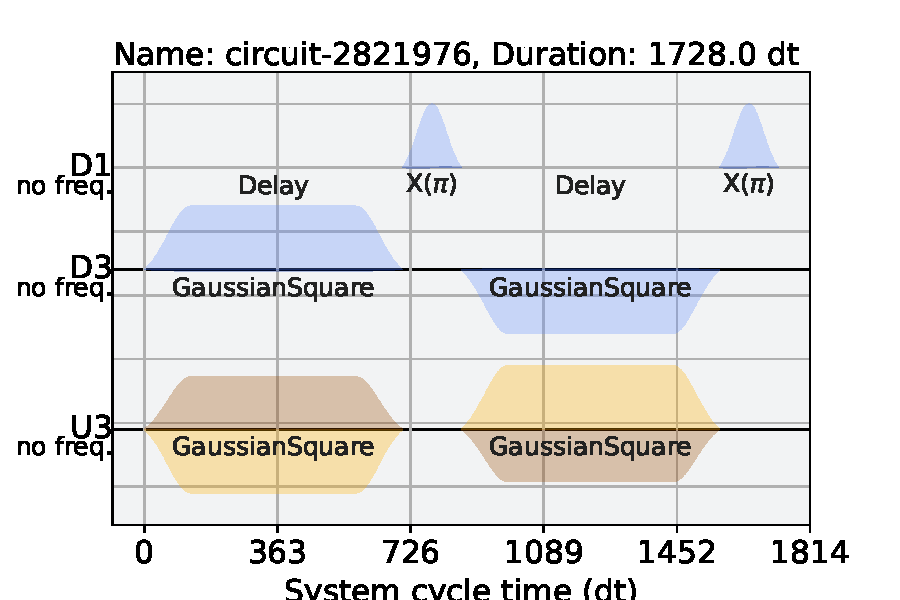
\includegraphics[scale=0.5]{demoEchoedCRPulse.pdf}
      \caption{Echoed cross resonance gate calibration for implementation of CNOT gates in IBM Quantum backends. Control qubit corresponds to index 1, whereas target qubit, to index 3. This figure represents a typical calibration for \textit{ibmq jakarta}.}
      \label{fig:echoedPulseQiskit}
    \end{figure}

  \subsection{Cross-resonance based transpilation of quantum includes}
  \label{subsec:CrossResonanceTranspilation}

    As mentioned before, IBM Quantum exposes a highly calibrated CNOT gates as entangling operations. However, in some instances, CNOT based circuit transpilation to microwave pulse schedules lead to execution times that are impossible to execute with high fidelity on current quantum devices. An example is time simulation of Majorana fermionic systems \cite{MajoranaSimulation}. A key insight towards performing pulse efficient implementation of quantum algorithms is to use the highly calibrated CNOT schedule exposed by IBM Quantum backends to perform cross resonance gates discussed on the previous section \cite{MajoranaSimulation, RXZPulseEfficient}. The details on the gaussian pulse scaling can be found on \cite{MajoranaSimulation}. The idea is to scale the area of the pulses in direct proportion to the angle of rotation of the cross resonance gate. Then, adjust the width, amplitude, and duration of the pulse accordingly. Through Qiskit SDK, it is possible to perform this calibration as discussed in the appendix of \cite{RXZPulseEfficient}.

    As pointed out on \cite{RXZPulseEfficient}, with calibrated cross resonance gates, it is possible to implement two qubit gates of the group

    \begin{equation}
      \hat{U}(\alpha, \beta, \gamma) = \mathrm{e}^{-\mathrm{i}(\alpha\hat{X}\hat{X} + \beta\hat{Y}\hat{Y} + \gamma\hat{Z}\hat{Z})}.
      \label{eq:CartanDecomp}
    \end{equation}

    \begin{figure}
    \centering
    \begin{quantikz}
        & \gate{H} & \gate[wires=2]{RZX(\alpha)} & \gate{H} & \gate{S^{\dagger}} & \gate{H} & \gate[wires=2]{RZX(\beta)} & \gate{H} & \gate{S} & \qw    & \gate[wires=2]{RZX(\gamma)} & \qw &\\
        & \qw      &                             & \qw      & \gate{S^{\dagger}} & \qw      &                            & \qw      & \gate{S} & \gate{H} &                                & \gate{H} &
    \end{quantikz}
    \caption{Circuit representation of efficient pulse implementation of unitary operation \ref{eq:CartanDecomp}, according to \cite{RXZPulseEfficient}. Each $RZX$ gate represents a cross resonance interaction with pulse schedule as in figure \ref{fig:echoedPulseQiskit}, with scaling performed as proposed in \cite{MajoranaSimulation}.}
\end{figure}

    As shown on \cite{RXZPulseEfficient} and \cite{MajoranaSimulation}, this type of algorithm transpilation leads to a significant relative error reduction for shorter pulse schedules, allowing time simulation of interesting physical systems. Benchmark test were made in comparison to the three CNOT decomposition depicted on figure \ref{fig:cartan3Cnot}. It was shown experimentally that the relative error can be decreased up to $50\%$ by implementing pulse efficient algorithms on current quantum devices \cite{RXZPulseEfficient}.



%%%%%%%%%%%%%%%%%%%%%%%%%%%%%%%%%%%%%%%%%%%%%%%%%%%%%%%%%%%%%%%%%%%%%%%%%%%%%%%%
%                          QUANTUM TIME SIMULATION                             %
%%%%%%%%%%%%%%%%%%%%%%%%%%%%%%%%%%%%%%%%%%%%%%%%%%%%%%%%%%%%%%%%%%%%%%%%%%%%%%%%
  \chapter{Quantum Time Simulation}
  \label{chap:qts}
  An introduction to quantum time simulation, as opposed to \textit{classical} time simulation of quantum systems is presented on \autoref{sec:qtsVcts}. After that, a generic framework for approximate quantum time evolution is presented on \autoref{sec:trotter} Finally, on \autoref{sec:hubbard}, quantum digital simulations of one-dimensional Hubbard models, carried out by Las Heras et. al. \cite{HubbardSimulLasHeras} and Barends et. al. \cite{HubbardSimul}, are discussed as immediate predecessors of this works.

\section{Quantum Time Simulation v. Classical Time Simulation}
\label{sec:qtsVcts}

  At the heart of simulation of quantum physical systems is solving Schrödinger's equation of motion \cite{Beck, Nielsen}:

  \begin{equation}
  \mathrm{i}
  \label{eq:SchEqn}\pdv{\ket{\psi}}{t} = \hat{H} \ket{\psi}
  \end{equation}

  Where $\hat{H}$ is the Hamiltonian that defines the interaction between the system's components, and perhaps its environment. In position representation, A one-dimensional system of spinless particles can be simulated by solving the equation

  \begin{equation}
  \mathrm{i}\pdv{\ket{\psi}}{t} = \Bigg[\sum_{i = 1}^{n} \frac{\hat{P}_i^2}{2m_i} + \hat{V}(x_1, x_2, \ldots, x_n)\Bigg] \ket{\psi}
  \end{equation}

  Supposed $\ket{\psi}$ represents an $n$-particle system state. Hence, a single particle dynamics can be determined by solving the equation

  \begin{equation}
  \mathrm{i}\pdv{\ket{\psi}}{t} = \Bigg[\frac{\hat{P}^2}{2m} + \hat{V}(x)\Bigg] \ket{\psi}
  \end{equation}

  A classical algorithm may use a fine discretization of position basis, in some spatial region $\mathit{S} = [0,L]$, with a basis of $N$ statevectors and a discretization step $\Delta x = L/(N-1)$. Such that

  \begin{equation}
    \ket{x} \text{ for } x \in S \rightarrow \ket{k \Delta x} \text{ for } k = 0,1,\ldots,N-1
  \end{equation}

  This scheme leads to a representation of any single particle position state as a linear combination of discrete statevectors

  \begin{equation}
    \ket{\psi(t)} = \sum_{k = 0}^{N-1} a_k(t) \ket{k \Delta x}
  \end{equation}

  Momentum operator could be approximated using finite difference formulas, thus leading to a system of coupled differential equation on the expansion coefficients $a_k$

  \begin{equation}
    \mathrm{i}\pdv{a_k}{t} = \sum_{l = 0}^{N} H_{kl} a_l
    \label{eq:MatrixSchr}
  \end{equation}

  Solution of equation \ref{eq:MatrixSchr}, given $a_k(0)$, would yield a complete knowledge of the particle's dynamics at any time. Typically, this would require diagonalization of the Hamiltonian matrix, $H_{kl}$. There are more efficient approaches than this, of course. For instance, Numerov integration. However, the goal of this example is to introduce quantum time simulation on a digital quantum computer as smoothly as possible.

  Time simulation on a digital quantum computer could be carried out in a very different way \cite{Strini, Nielsen}. A schematic is presented on figure \ref{fig:timevolslice}. Pretty much in the same way as in the naïve example discussed before, position basis may be discretized. Nevertheless, this time the coefficients would be encoded directly as the amplitudes of the statevector of an $n$-qubit computer. It is readily seen that to achieve a discretization with $N$ system statevectors, only $\mathcal{O}(\log{N})$ qubits are needed. Although not very significant for a single particle, this illustrates that quantum computers have inherent exponential advantage over classical computers in terms of space resources. Instead of diagonalizing the Hamiltonian, digital quantum time simulation relies on the direct solution

  \begin{equation}
    \ket{\psi(t)} = \exp(-\mathrm{i}\int_{t_0}^t \hat{H}(t)dt)\ket{\psi(0)}
    \label{eq:UnitaryEvolution}
  \end{equation}

  Which for time-independent Hamiltonians reduces to

  \begin{equation}
    \ket{\psi(t)} = \mathrm{e}^{-\mathrm{i}(t - t_0) \hat{H}}\ket{\psi(0)}
    \label{eq:UnitaryEvolutionNoTime}
  \end{equation}

  In the naïve example considered until now, time evolution with a digital quantum computer amounts to computing unitary operator ($t_0 = 0$)

  \begin{equation}
    \hat{U}(t) = \mathrm{e}^{-\mathrm{i}t \frac{\hat{P}^2}{2m}}\mathrm{e}^{-\mathrm{i}t \hat{V}(x)} + \mathcal{O}(t^2)
  \end{equation}

  Using Baker-Haussdorf formulae, or a Suzuki-Trotter scheme of higher order, better expressions for the time evolution operator of the system may be obtained. Notice that operator

  \[
  \hat{U}_P = \mathrm{e}^{-\mathrm{i}t \frac{\hat{P}^2}{2m}}
  \]

  Is efficiently computable, using the Quantum Fourier Transform Algorithm:

  \[
  \hat{U}_P = QFT\mathrm{e}^{-\mathrm{i}t \frac{\hat{x}^2}{2m}}QFT^{\dagger}
  \]

  Therefore, if operator

  \[
  \hat{U}_V = \mathrm{e}^{-\mathrm{i}t \hat{V}(x)}
  \]

  Is efficiently computable, time simulation on a quantum computer might be more resource-friendly, both in terms of space and time, than common simulation using classical computers. Only theoretical constraints are error bounds for a given simulation time interval. Given simulation time and error bound, a time slice $dt$ is fixed, and thus repeated application of operator $\hat{U}(dt)$ evolves a single particle state from some initial state $\ket{\psi(0)}$, to state $\ket{\psi(t)}$.

  \begin{figure}
    \centering
    \begin{quantikz}
      \lstick[wires=4]{$\ket{\psi(0)}$} & \gate[wires=4]{QFT^{\dagger}} & \gate[wires=4]{\mathrm{e}^{-\mathrm{i}t \frac{\hat{x}^2}{2m}}} & \gate[wires=4]{QFT^{\dagger}} & \gate[wires=4]{\mathrm{e}^{-\mathrm{i}t \frac{\hat{V}(x)}{2m}}} & \qw  \rstick[wires=4]{$\ket{\psi(t)}$} \\
                                        &                               &                                                              &                               &                                                                 & \qw                                    \\
                                        &                               &                                                              &                               &                                                                 & \qw                                    \\
                                        &                               &                                                              &                               &                                                                 & \qw                                    \\
    \end{quantikz}
    \caption{Time evolution slice for a single particle state on a digital quantum computer. This step should be repeated several times, with a time step $dt$, which depends upon the desired error bound and spatial discretization.}
    \label{fig:timevolslice}
  \end{figure}

  In summary, rather than using physical bits to encode the expansion coefficients of a particle's state, like on a classical computer, a quantum algorithm relies on the nature of qubits to encode directly such a state. This leads to an exponential reduction in the space complexity of the problem. Furthermore, multi-qubit gates can be used to implement unitary evolution, without the explicit need of matrix diagonalization. Thus leading to a potentially faster evolution simulation. For a simple system like this, codification of the information of all expansion coefficients would require at least $2N$ reals parameters. Furthermore, diagonalization of the Hamiltonian matrix, $H_{kl}$, would require $\mathcal{O}(N^2)$ computational steps. As a result, the simulation advantage posed by quantum computation seems unnecessary. Also, there are numerous efficient classical algorithms for solving Schrodinger's time dependent equation, such as Numerov or Runge-Kutta integration. However, this example illustrates the difference between classical simulation and quantum simulation using a digital quantum computer, and some of the possible advantages of quantum time simulation using the former type of information processors.

  For a one-dimensional system of several particles, equation \ref{eq:MatrixSchr} can be generalized easily. However, the number of coefficients required to describe a statevector in a discrete basis would grow exponentially with the number of particles. As well as matrix Hamiltonian size. As a result, simulation of time dynamics on a classical computer results impractical. Therefore, quantum time simulation of multi-particle systems is an application to which digital quantum computers may represent a practical advantage. In the following sections, common techniques for quantum time simulation in digital computers are presented. In particular, simple approximation formulas are discussed and compared. 

  %% Here I would have to talk more about...

\section{Common Approximation Schemes for Unitary Evolution}
\label{sec:trotter}

  Consider a system of $N$ components, whose Hamiltonian can be expressed as a sum of local Hamiltonians (i. e. that model interaction between at most $C$ components) \cite{Nielsen,LloydNature}

  \begin{equation}
    \hat{H} = \sum_{k = 1}^{L} \hat{H}_k
    \label{eq:SparseHam}
  \end{equation}

  Where $L$ is some polynomial on the number of system components. In general, $[\hat{H}_i,\hat{H}_j] \neq 0$, and thus

  \begin{equation}
    \mathrm{e}^{-\mathrm{i}\hat{H}t} \neq \prod_{k = 1}^{L} \mathrm{e}^{-\mathrm{i}\hat{H}_kt}
    \label{eq:CommuteUnit}
  \end{equation}

  Many systems are described by local interactions, for instance, electrons in a solid material or magnetic moments in a lattice. In several cases, local interaction Hamiltonians are non-commuting, and thus approximation methods are necessary for performing time evolution. In this section, schemes for approximating unitary evolution of a quantum system are discussed.

  \subsection{Trotter Formulas}

  Consider operators $\hat{H}_1$, $\hat{H}_2$, with $[\hat{H}_1,\hat{H}_2] \neq 0$. By definition

  \begin{align}
    \mathrm{e}^{-\mathrm{i}\hat{H}_1 t} & = \sum_{m = 0}^{\infty} \frac{(-\mathrm{i}t)^m}{m!}\hat{H}_1^m \\
    \mathrm{e}^{-\mathrm{i}\hat{H}_2 t} & = \sum_{l = 0}^{\infty} \frac{(-\mathrm{i}t)^l}{l!}\hat{H}_2^l
    \label{eq:ExpSeries}
  \end{align}

  It is readily shown that

  \begin{equation}
    \mathrm{e}^{-\mathrm{i}\hat{H}_1 t}\mathrm{e}^{-\mathrm{i}\hat{H}_2 t} = \sum_{k = 0}^{\infty} \frac{(-\mathrm{i}t)^k}{k!} \Bigg[\sum_{m = 0}^k \binom{k}{m} \hat{H}_1^m \hat{H}_2^{k-m}\Bigg]
    \label{eq:ExpProdExact}
  \end{equation}

  Fon non-commuting operators, it is so that

  \begin{equation}
    \sum_{m = 0}^k \binom{k}{m} \hat{H}_1^m \hat{H}_2^{k-m} = (\hat{H}_1 + \hat{H}_2)^k + f_k(\hat{H}_1,\hat{H}_2)
    \label{eq:BinomialTheorem}
  \end{equation}

  Where $f_k(\hat{H}_1,\hat{H}_2)$ is a function of the commutator of the operators. Since $f_1(\hat{H}_1,\hat{H}_2) = 0$, it is so that

  \begin{equation}
    \mathrm{e}^{-\mathrm{i}\hat{H}_1 t}\mathrm{e}^{-\mathrm{i}\hat{H}_2 t} = \mathrm{e}^{-\mathrm{i}(\hat{H}_1 + \hat{H}_2) t} + \mathcal{O}(t^2)
    \label{eq:O2Approx}
  \end{equation}

  If $|t| \ll 1$, the product of the exponential operators estimate the evolution operator with an error $\mathcal{O}(t^2)$. In the general case, it must be noted that

  \begin{equation}
    \mathrm{e}^{-\mathrm{i}\sum_{k = 0}^L \hat{H}_k t} = \hat{1} + (-\mathrm{i}t)\sum_{k = 0}^L \hat{H}_k + \frac{(-\mathrm{i}t)^2}{2} \Bigg[\sum_{k = 0}^L \hat{H}_k^2 + 2 \sum_{j > k}\hat{H}_k \hat{H}_j\Bigg] + \mathcal{O}(t^3)
    \label{eq:TrotterFormula}
  \end{equation}

  In consequence, a unitary evolution operator with local interactions may be approximated, to quadratic order, by the exponential product

  \begin{equation}
    \mathrm{e}^{-\mathrm{i}\sum_{k = 0}^L \hat{H}_k t} = \prod_{k = 1}^{L} \mathrm{e}^{-\mathrm{i}\hat{H}_kt} + \mathcal{O}(t^2)
    \label{eq:2ndOrderTrotter}
  \end{equation}

  In some instances, quadratic approximations may be enough. In his seminal paper, Lloyd presents this quadratic approximation for simulation of quantum systems with local interaction \cite{LloydNature}. Also, Las Heras et. al. simulate a Hubbard Hamiltonian with up to 4 fermionic modes using second order approximations to unitary evolution \cite{HubbardSimul, HubbardSimulLasHeras}. However, in following sections, higher-order approximation schemes are discussed, based upon equation \ref{eq:TrotterFormula}.

  \subsection{Some Cubic Order Schemes}

  The first cubic order approximation discussed is the so called Baker-Haussdorf formulae \cite{Nielsen}. By series expansion, it can be shown that

  \begin{align*}
    \mathrm{e}^{-\mathrm{i}\hat{H}_1t}\mathrm{e}^{-\mathrm{i}\hat{H}_2t}\mathrm{e}^{-\mathrm{i}[\hat{H}_1,\hat{H}_2]t^2} = & \hat{1} + (-\mathrm{i}t) (\hat{H}_1 + \hat{H}_2) \\
    & + \frac{(-\mathrm{i}t)^2}{2}(\hat{H}_1^2 + \hat{H}_2^2 + \hat{H}_1\hat{H}_2 + \hat{H}_2\hat{H}_1) + \mathcal{O}(t^3) \\
    = & \mathrm{e}^{-\mathrm{i}(\hat{H}_1 + \hat{H}_1)t} + \mathcal{O}(t^3)
    \label{eq:Hausdorf1}
  \end{align*}

  Although useful in case of operators that constitute a Lie algebra, the formulae above may not be enough in other instances. A more general approximation formulae is

  \begin{equation}
    \mathrm{e}^{-\mathrm{i}t\sum_{l = 0}^{L-1}\hat{H}_l} = \Bigg(\prod_{l = 0}^{L-1}\mathrm{e}^{-\mathrm{i}\hat{H}_l\frac{t}{2}}\Bigg)\Bigg(\prod_{l = L-1}^{0}\mathrm{e}^{-\mathrm{i}\hat{H}_l\frac{t}{2}}\Bigg) + \mathcal{O}(t^3)
    \label{eq:Suzuki0}
  \end{equation}

  This can be deduced directly from the identity

  \begin{equation}
    \mathrm{e}^{-\mathrm{i}\sum_{l = 0}^{2L-1} \hat{K}_l t} = \hat{1} + (-\mathrm{i}t)\sum_{l = 0}^{2L-1} \hat{K}_l + \frac{(-\mathrm{i}t)^2}{2} \Bigg[\sum_{l = 0}^{2L-1} \hat{K}_l^2 + 2 \sum_{j > l}\hat{K}_l \hat{K}_j\Bigg] + \mathcal{O}(t^3)
    \label{eq:TrotterFormula1}
  \end{equation}

  With the identifications

  \begin{equation}
    \hat{K}_l = \hat{K}_{2L-1-l} = \frac{\hat{H}_l}{2}
    \label{eq:Identifications}
  \end{equation}

  And the following observations

  \begin{equation}
    \begin{gathered}
      \sum_{l = 0}^{2L-1} \hat{K}_l^2 = \frac{1}{2}\sum_{l = 0}^{L-1} \hat{H}_l^2 \\
      2\sum_{l' > l} \hat{K}_{l} \hat{K}_{l'} = \frac{1}{2}\sum_{l = 0}^{L-1} \hat{H}_l^2 + \sum_{l'> l} \Bigg( \hat{H}_{l} \hat{H}_{l'} + \hat{H}_{l'} \hat{H}_{l}\Bigg)\\
      \Bigg(\sum_{l = 0}^{L-1} \hat{H}_l \Bigg)^2 = \sum_{l = 0}^{L-1} \hat{H}_l^2 + \sum_{l'> l} \Bigg( \hat{H}_{l} \hat{H}_{l'} + \hat{H}_{l'} \hat{H}_{l}\Bigg)\\
    \end{gathered}
  \end{equation}

  \subsection{Suzuki - Trotter Scheme}
  This scheme is a higher order approximation to an evolution operator, that works iteratively on top of the approximation given by equation \ref{eq:Suzuki0}. Define \cite{SuzukiFormula, BerryErrorBounds}

  \begin{equation}
    \hat{S}_2(\lambda) = \prod_{l = 0}^{L-1} \mathrm{e}^{\frac{\lambda}{2}\hat{H}_l} \prod_{l = L-1}^{0} \mathrm{e}^{\frac{\lambda}{2}\hat{H}_l}
    \label{eq:SuzukiInit}
  \end{equation}

  Then, for $k > 1$, the following recursion relation is defined

  \begin{equation}
    \hat{S}_{2k}(\lambda) = [\hat{S}_{2k-2}(p_k\lambda)]^2 \hat{S}_{2k-2}((1 - 4 p_k)\lambda) [\hat{S}_{2k-2}(p_k\lambda)]^2
    \label{eq:SuzukiRecursion}
  \end{equation}

  Where coefficients $p_k$ are defined as

  \begin{equation}
    p_k = \frac{1}{4 - 4^{\frac{1}{2k-1}}}
    \label{eq:pk}
  \end{equation}

  It has been shown by Suzuki that \cite{SuzukiFormula}

  \begin{equation}
    \mathrm{e}^{-\mathrm{i}t \sum_{l = 0}^{L-1} \hat{H}_l} = \hat{S}_{2k}(-\mathrm{i}t) + \mathcal{O}(t^{2k+1})
  \end{equation}

  On \cite{BerryErrorBounds}, Barry et. al. show that Suzuki-Trotter schemes can efficiently simulate sparse Hamiltonians, such as the ones considered in this work. As a matter of fact, they have shown that the number of exponentials ($N_{\text{exp}}$) required to simulate time evolution of a system during a time interval $t > 0$, with error bounded by $\epsilon > 0$, is such that

  \begin{equation}
    N_{\text{exp}} \leq 2L5^{2k}(L\tau)^{1+1/2k}/\epsilon^{1/2k}
  \end{equation}

  Where $\tau = \left\Vert \hat{H} \right\Vert t$, $2k$ is the order of a Suzuki-Trotter iteration, and $\epsilon \leq 1 \leq 2L5^{2k}$. Notice that by choosing a sufficiently high order, a Suzuki-Trotter scheme can emulate time evolution with almost linear complexity in time.

  In most cases, simulation of a quantum system by a digital quantum computer requires mapping its Hilbert space to a $2^M$-dimensional Hilbert space. In that case, the number of qubits required for simulation would be $M$. Clearly, all quantum operators in the simulated system's space should be mapped to operators on an $M$-qubit space, which would then be approximated by a universal set of gates. In the following section, demonstrations of this approach to the study of the Hubbard Model and the Electronic structure problem are introduced.

\section{Time Simulation of Spin 1/2 Models}
\label{sec:hubbard}
  
  On section \ref{sec:qtsVcts}, a comparison between classical time simulation and quantum time simulation was introduced. In particular, a scheme for integrating Schrödinger's equation for a $n$-particle system was proposed. This section introduces examples of simulation of Hamiltonians such as

  \begin{equation}
    \hat{H} = \sum_{\langle i,j \rangle} J_{ij}^{(x)} \hat{X}_i \hat{X}_j + J_{ij}^{(Y)} \hat{Y}_i \hat{Y}_j + J_{ij}^{(Z)} \hat{Z}_i \hat{Z}_j + \sum_i h_i^{(X)} \hat{X}_i + h_i^{(Y)} \hat{Y}_i + h_i^{(Z)} \hat{Z}_i
    \label{eq:HeisenbergHamiltonian}
  \end{equation}

  Defined over an arbitrary spin graph, and considering nearest neighbor interaction. Most of them are related to work from Las Heras et. al. \cite{HubbardSimul,HubbardSimulLasHeras} and Y. Salathé \cite{HeisenbergSimulLasHeras}. In this section, the importance of simulating such systems is discussed. Furthermore, the examples considered here are further generalized in following chapters to simulate any system whose Hamiltonian is of the shape of eq. \ref{eq:HeisenbergHamiltonian}, and its limitations are exemplified.

  \subsection{Digital simulation of two-spin models}

  As a first example, simulation of two-spin models carried out by Y. Salathé et. al. \cite{HeisenbergSimulLasHeras} are presented. In their work, a superconducting chip with two trasmon qubits is used to simulate two-spin interaction described by the Hamiltonian

  \begin{equation}
    \hat{H}_{1,2}^{x,y} = \frac{J}{2} \bigg( \hat{X}_1 \hat{X}_2 + \hat{Y}_1 \hat{Y}_2 \bigg)
    \label{eq:fundamentalSlatheGate}
  \end{equation}

  This means that they where able to evolve the qubits' state during time $t$, using microwave pulses on the chip, with unitary dynamics governed by Hamiltonian \ref{eq:fundamentalSlatheGate}. It is easy to see that by performing single qubit rotations, it is possible to emulate more complicated dynamics, for instance, an isotropic XYZ interaction

  \begin{equation}
    \hat{H}_{1,2}^{x,y,z} = J \bigg( \hat{X}_1 \hat{X}_2 + \hat{Y}_1 \hat{Y}_2 + \hat{Z}_1 \hat{Z}_2 \bigg)
    \label{eq:XYZSalathe}
  \end{equation}

  An algorithm for simulating time dynamics under Hamiltonian \ref{eq:XYZSalathe} is presented on fig. \ref{fig:salathe-xyz}. The reported state fidelities of the evolution process are above $82\%$. It must be noted that, since all terms of the Hamiltonian commute, the evolution of the two qubit state is exact, and only limited by hardware. In addition to that, an algorithm for simulating the Ising model with transverse homogeneous magnetic field was proposed (see fig. \ref{fig:salathe-ising}).
  
  \begin{equation}
    \hat{H}_I = J \hat{X}_1 \hat{X}_2 + \frac{B}{2}\bigg(\hat{Z}_1 + \hat{Z}_2 \bigg)
    \label{eq:IsingSlathe}
  \end{equation}

  Notice that this Hamiltonian is composed of local parts that do not commute with one another (spin interaction and field interaction), thus an approximate evolution scheme is needed to simulate time evolution. In their work, Salathé et. al. \cite{HeisenbergSimulLasHeras} used a second order trotterization (see eq. \ref{eq:2ndOrderTrotter}). Furthermore, a noise model was proposed to take into account the fact that decoherence and gate errors limit the expected precision of a trotterization scheme. The results show that the main source of error is the infidelity of the two-qubit gate implementation of the XY interaction (eq. \ref{eq:fundamentalSlatheGate}).

  \subsection{Digital simulation of Hubbard models}

  As a second example, the work of las Heras et. al. is considered\cite{HubbardSimulLasHeras}. The authors simulated instances of the quintessential Hubbard Hamiltonian

  \begin{equation}
    \hat{H}_H = -V \sum_{\langle i,j\rangle} (\hat{b}_i^{\dagger}\hat{b}_j + \hat{b}_j^{\dagger}\hat{b}_i) + U \sum_i \hat{n}_{i\uparrow}\hat{n}_{i\downarrow}
    \label{eq:HubbardHamiltonian}
  \end{equation}

  Where $\hat{b}_i$ represent fermionic-mode annihilation operators (for spin-up or spin-down particles), and $\hat{n}_{i\uparrow},\hat{n}_{i\uparrow}$, fermionic-mode occupation number operators. This was done using the Jordan-Wigner mapping, which transforms fermionic operators to qubit operators. The rule is that each occupation mode is mapped directly to the state of a qubit, so that its state encodes the occupation number of the mode in the computational basis. Fermionic annihilation operators are mapped directly following the rule \cite{Mastersthesis}

  \begin{equation}
    \hat{b}_i = \hat{\sigma}_i^{+} \otimes \Bigg(\bigotimes_{k=0}^{N} \hat{Z}_k \Bigg)
    \label{eq:JWT}
  \end{equation}

  Where it is assumed that a linear indexing of the modes is used, even for different spin values. The authors considered models with up to four modes. In particular, they showed that the mapping of a two-mode Hubbard Hamiltonian like eq. \ref{eq:HubbardHamiltonian} leads to a qubit Hamiltonian

  \begin{equation}
    \hat{H}_H = \frac{V}{2}\big(\hat{X}_1 \hat{X}_2 + \hat{Y}_1 \hat{Y}_2\big) + \frac{U}{4} \big(\hat{Z}_1 \hat{Z}_2 + \hat{Z}_1 + \hat{Z}_2\big)
    \label{eq:TwoModeHubbard}
  \end{equation}

  The authors used a superconducting chip for simulating time dynamics governed by Hamiltonian \ref{eq:TwoModeHubbard}. The quantum algorithm is represented on figure \ref{fig:heras-hubbard}. It was used to simulate time evolution with an initial state
  
  $$
  \ket{\psi_0} = \frac{1}{\sqrt{2}}(\ket{0} + \ket{1}) \otimes \ket{0}
  $$

  With $V=U=1$, for a time $t=5$. The results showed that process errors in the implementation of a Trotter step leads to a linear decrease in state fidelity with the number of steps. This is an important factor to consider when implementing Suzuki-Trotter schemes for simulating time evolution. However, their simulations were able to capture the overall dynamics, obtaining fidelities near $90\%$ with a small number of Trotter steps. Three and four mode anisotropic models were simulated as well, obtaining similar results \cite{HubbardSimulLasHeras}.

  It has been shown by Reiner \cite{Mastersthesis} that a one dimensional Hubbard model (eq. \ref{eq:HubbardHamiltonian}) can be mapped to a qubit Hamiltonian of the type \ref{eq:HeisenbergHamiltonian}, by means of the Jordan Wigner mapping. Thus, by generalizing the quantum algorithms presented on these examples, it is possible to study correlation phenomena on metallic solids efficiently, in contrast to current classical simulation methods \cite{Mastersthesis,HubbardOriginal}. In following chapters,  general routines for simulating evolution under Hamiltonian \ref{eq:HeisenbergHamiltonian} are presented, and quantum time evolution is showcased as a tool for studying magnetic properties of solids. Moreover, a discussion of the influence of decoherence and errors in the implementation is carried out, thus presenting the limitations of Suzuki-Trotter schemes for simulating many-body systems.

  \begin{figure}
    \centering
    \begin{subfigure}[b]{1.0\textwidth}
        \centering
        \caption{}
        \begin{quantikz}
            \lstick[wires=2]{$\ket{\psi(0)}$} & \gate[wires=2]{\mathrm{e}^{-\mathrm{i}\hat{H}_{1,2}^{x,y}t}} & \gate{R_{\hat{x}, -\pi/2}} & \gate[wires=2]{\mathrm{e}^{-\mathrm{i}\hat{H}_{1,2}^{x,y}t}} & \gate{R_{\hat{x}, \pi/2}} & \gate{R_{\hat{y}, -\pi/2}} & \gate[wires=2]{\mathrm{e}^{-\mathrm{i}\hat{H}_{1,2}^{x,y}t}} &  \gate{R_{\hat{y}, \pi/2}} & \qw \rstick[wires=2]{$\ket{\psi(t)}$}\\
             & & \gate{R_{\hat{x}, -\pi/2}} & & \gate{R_{\hat{x}, \pi/2}} & \gate{R_{\hat{y}, -\pi/2}} & & \gate{R_{\hat{y}, \pi/2}} & \qw
        \end{quantikz}
        \label{fig:salathe-xyz}
    \end{subfigure}
    \vfill
    \begin{subfigure}[b]{1.0\textwidth}
        \centering
        \caption{}
        \begin{quantikz}
            \gate{R_{\hat{x}, \pi}} & \gate[wires=2]{\mathrm{e}^{-\mathrm{i}\hat{H}_{1,2}^{x,y}\frac{t}{N}}} & \gate{R_{\hat{x}, -\pi}} & \gate[wires=2]{\mathrm{e}^{-\mathrm{i}\hat{H}_{1,2}^{x,y}\frac{t}{N}}} &  \gate{R_{\hat{z}, \frac{t}{N}}} \\
            \qw & & \qw & & \gate{R_{\hat{z}, \frac{t}{N}}}
        \end{quantikz}
        \label{fig:salathe-ising}
    \end{subfigure}
    \begin{subfigure}[b]{1.0\textwidth}
        \centering
        \caption{}
        \begin{quantikz}
            \gate{R_{\hat{y}, \pi/2}} & \gate[wires=2]{\mathrm{e}^{-i\frac{\phi_{xx}}{2}\hat{Z}\otimes\hat{Z}}} & \gate{R_{\hat{y}, -\pi/2}} & \gate{R_{\hat{x}, -\pi/2}} & \gate[wires=2]{\mathrm{e}^{-i\frac{\phi_{yy}}{2}\hat{Z}\otimes\hat{Z}}} & \gate{R_{\hat{x}, \pi/2}} & \gate[wires=2]{\mathrm{e}^{-i\frac{\phi_{zz}}{2}\hat{Z}\otimes\hat{Z}}} & \gate{R_{\hat{z}, \phi_z}} \\
            \gate{R_{\hat{y}, \pi/2}} & & \gate{R_{\hat{y}, -\pi/2}} & \gate{R_{\hat{x}, -\pi/2}} & & \gate{R_{\hat{x}, \pi/2}} & & \gate{R_{\hat{z}, \phi_z}}
        \end{quantikz}
        \label{fig:heras-hubbard}
    \end{subfigure}
    \caption{(a) Digital quantum algorithm for simulating time dynamics of isotropic XYZ model according to \cite{HeisenbergSimulLasHeras}. Notice that commutation of $\hat{X}_1\hat{X}_2$, $\hat{Y}_1\hat{Y}_2$, and $\hat{Z}_1\hat{Z}_2$ implies that the resulting dynamics is exact up to hardware errors. (b) Trotter step for simulating of the Ising model with a transverse magnetic field. This step is repeated $N$ times to evolve over a time interval $t$ \cite{HeisenbergSimulLasHeras}. (c) Trotter step for simulating a two-mode Hubbard model. Here $\phi_{zz} = \phi_z = Ut/2N$ and $\phi_{xx} = \phi_{yy} = Ut/2N$ \cite{HubbardSimulLasHeras}.}
    \label{fig:salathe-circuits}
\end{figure}

  

  

%%%%%%%%%%%%%%%%%%%%%%%%%%%%%%%%%%%%%%%%%%%%%%%%%%%%%%%%%%%%%%%%%%%%%%%%%%%%%%%%
%                          ANISOTROPIC SPIN CHAIN                              %
%%%%%%%%%%%%%%%%%%%%%%%%%%%%%%%%%%%%%%%%%%%%%%%%%%%%%%%%%%%%%%%%%%%%%%%%%%%%%%%%
  \chapter{Anisotropic Spin Chain}
  \label{chap:main}
  This chapter introduces time simulation algorithms for Hamiltonian \ref{eq:HeisenbergHamiltonian}. First a trotterization scheme is introduced, and its advantages are discussed for simulating certain types of graphs or lattices. Relations between discretization step, evolution time and evolution error are computed and discussed in order to establish disadvantages of execution on current (noisy) quantum devices. Then, three possible implementation strategies are introduced: 1) a direct transpilation of circuits proposed by Las Heras et. al. \cite{HubbardSimulLasHeras}, 2) a basis-efficient transpilation relying on commutation properties of local Hamiltonians \footnote{The work was performed at early stages independently of that on \cite{BellUniversalCartan}. However, the insights are identical and thus the author is compelled to refer to this previous work. It is clear, however, that the mentioned reference considers the problem of universal two qubit gates which, albeit related to the specific problem of the present dissertation, is a quite different approach. This dissertation uses the results derived to solve a specific time evolution problem with potential application to specific areas of solid state physics and physical chemistry.}, and 3) a pulse-efficient transpilation based on cross-resonance interaction. Finally, the three algorithms are tested using a three-qubit Hamiltonian. Time evolution of probability density, and of single-qubit Pauli operators' expected values, are computed. Whereas probability density fidelity and state fidelity are used as quantitative indicators.

\section{Trotterization And Time Evolution}
\label{sec:MainTrotterScheme}

  Consider the multiple spin Hamiltonian

  \begin{equation}
    \hat{H} = \sum_{\langle i,j \rangle} J_{ij}^{(X)} \hat{X}_i \hat{X}_j + J_{ij}^{(Y)} \hat{Y}_i \hat{Y}_j + J_{ij}^{(Z)} \hat{Z}_i \hat{Z}_j + \sum_i h_i^{(X)} \hat{X}_i + h_i^{(Y)} \hat{Y}_i + h_i^{(Z)} \hat{Z}_i,
    \label{eq:HeisenbergHamiltonian2}
  \end{equation}

  \noindent defined over an arbitrary graph. The shape already suggests that the Hamiltonian above can be decomposed in local interactions of the shape

  \begin{gather}
    \hat{H}_{ij} = J_{ij}^{(X)} \hat{X}_i \hat{X}_j + J_{ij}^{(Y)} \hat{Y}_i \hat{Y}_j + J_{ij}^{(Z)} \hat{Z}_i \hat{Z}_j, \\
    \hat{H}_{i} = h_i^{(X)} \hat{X}_i + h_i^{(Y)} \hat{Y}_i + h_i^{(Z)} \hat{Z}_i,
    \label{eq:HamiltonianDecomposition}
  \end{gather}

  \noindent such that

  \begin{equation}
    \hat{H} = \sum_{\langle i,j \rangle} \hat{H}_{ij} + \sum_i \hat{H}_i.
  \end{equation}

  This leads to a direct second order trotterization of the shape

  \begin{equation}
    \mathrm{e}^{-\mathrm{i}\hat{H}\Delta t} \approx \prod_{\langle i,j \rangle} \mathrm{e}^{-\mathrm{i}\hat{H}_{i,j}\Delta t} \prod_{i} \mathrm{e}^{-\mathrm{i}\hat{H}_i \Delta t} + \mathcal{O}(\Delta t^2).
    \label{eq:HamiltonianTrotterization}
  \end{equation}

   \noindent Interactions associated to disjoint edges commute, and thus can be simulated simultaneously. Hence, an advantage of this approach to time evolution is that by partitioning the graph on mutually disjoint sets, several terms can be implemented in parallel on actual quantum devices. This approach is implemented in the present work. This parallelism is illustrated for a spin chain in figure \ref{fig:spinChainCircuit}. It can be noticed that the circuit depth of the trotter step of three or more spins with chain topology is independent of the number of spins. As a result, time complexity only increases with the desired time discretization, which correlates with the error in the time simulation approximation. 
  
  Another interesting feature, as shown in figure \ref{fig:spinChainCircuit}, is that it is possible to perform third order time evolution using the first iteration of Suzuki-Trotter scheme with roughly the same time complexity as the second order trotterization. To illustrate this point more precisely, consider the Hamiltonian

  \begin{equation}
    \hat{H} = \sum_{i=0}^{\mathcal{N}-2} \hat{H}_{i,i+1},
    \label{eq:ChainHamiltonian}
  \end{equation}

  \noindent where $\hat{H}_{i,j}$ is defined as on equation \ref{eq:HamiltonianDecomposition}. It is straightforward to see that the second order evolution corresponds to the approximation

  \begin{equation}
    \mathrm{e}^{-\mathrm{i}\hat{H}\Delta t} \approx \prod_{i \text{ even}} \mathrm{e}^{-\mathrm{i}\hat{H}_{i,i+1}t} \prod_{i \text{ odd}} \mathrm{e}^{-\mathrm{i}\hat{H}_{i,i+1}t} + \mathcal{O}(\Delta t^2).
    \label{eq:HamiltonianTrotterization}
  \end{equation}

  \noindent For this particular system, denote

  \begin{gather}
    \hat{A}(\Delta t) = \prod_{i \text{ even}} \mathrm{e}^{-\mathrm{i}\hat{H}_{i,i+1}t}, \\
    \hat{B}(\Delta t) = \prod_{i \text{ odd}} \mathrm{e}^{-\mathrm{i}\hat{H}_{i,i+1}t},
    \label{eq:ChainOpsTrotter}
  \end{gather}

  \noindent such that

  \begin{equation}
    \mathrm{e}^{-\mathrm{i}\hat{H}\Delta t} \approx \hat{A}(\Delta t) \hat{B}(\Delta t) + \mathcal{O}(\Delta t^2).
    \label{eq:HamiltonianTrotterization}
  \end{equation}

  Simulation over a time $t = M \Delta t$ yields

  \begin{equation}
    \mathrm{e}^{-\mathrm{i}\hat{H}t} \approx \bigg( \hat{A}(\Delta t) \hat{B}(\Delta t) \bigg)^{M}.
    \label{eq:HamiltonianTrotterization}
  \end{equation}

  The third order scheme may be implemented using Suzuki-Trotter zeroth order evolution (eq. \ref{eq:Suzuki0}), yielding the following finite time approximation

  \begin{equation}
    \begin{aligned}
      \mathrm{e}^{-\mathrm{i}\hat{H}t} \approx & \bigg( \hat{A}(\Delta t/2) \hat{B}(\Delta t) \hat{A}(\Delta t/2) \bigg)^{M} \\
    = &  \hat{A}(\Delta t/2) \bigg( \hat{B}(\Delta t) \hat{A}(\Delta t) \bigg)^{M-1} \hat{B}(\Delta t) \hat{A}(\Delta t/2) \\
    = & \hat{A}(\Delta t/2) \hat{B}(\Delta t) \bigg( \hat{A}(\Delta t) \hat{B}(\Delta t) \bigg)^{M-1} \hat{A}(\Delta t/2).
    \label{eq:HamiltonianTrotterization}
    \end{aligned}
  \end{equation}

  It can be seen that the \textit{power} operator (the one with a power in the approximation unitary) on each scheme can be implemented in the same fashion on a quantum circuit. Hence, both second order and third order schemes have roughly the same time complexity when implemented on quantum devices. This optimization is taken into account during implementation on IBM Quantum backends.
  
  \begin{figure}
    \centering
    \begin{quantikz}
        & \gate[wires=2]{\mathrm{e}^{-\mathrm{i}\hat{H}_{0,1}\Delta t}} & \qw & \gate{\mathrm{e}^{-\mathrm{i}\hat{H}_{0}\Delta t}} & \qw \\
        & \qw & \gate[wires=2]{\mathrm{e}^{-\mathrm{i}\hat{H}_{1,2}\Delta t}} & \gate{\mathrm{e}^{-\mathrm{i}\hat{H}_{1}\Delta t}} & \qw \\
        & \gate[wires=2]{\mathrm{e}^{-\mathrm{i}\hat{H}_{2,3}\Delta t}} & \qw & \gate{\mathrm{e}^{-\mathrm{i}\hat{H}_{2}\Delta t}} & \qw \\
        & \qw & \gate[wires=2]{\mathrm{e}^{-\mathrm{i}\hat{H}_{3,4}\Delta t}} & \gate{\mathrm{e}^{-\mathrm{i}\hat{H}_{1}\Delta t}} & \qw \\
        & \qw & \qw  &      \gate{\mathrm{e}^{-\mathrm{i}\hat{H}_{4}\Delta t}} & \qw
    \end{quantikz}
    \caption{Trotter step for simulating a spin chain. Notice that spin-spin terms that do not share a graph point can be evolved in parallel. A greedy algorithm can be used to determine a possible, if not optimal, scheme for simulating spin-spin interactions on parallel.}
    \label{fig:spinChainCircuit}
\end{figure}

  \subsection{Limitations of the Scheme for Time Evolution}
  \label{subsec:TrotterDynamics}

    There are some intrinsic limitations to quantum time simulation using Trotter schemes. To exemplify this, consider an isotropic $\mathcal{N}$-spin chain Hamiltonian, with only two-spin interaction given by

    \begin{equation}
      \hat{H}_{ij} = \frac{1}{2} \hat{X}_i \hat{X}_j + \hat{Y}_i \hat{Y}_j + \frac{1}{4} \hat{Z}_i \hat{Z}_j.
      \label{eq:FloquetHamiltonian}
    \end{equation}

    Consider an initial state $\ket{\psi_0} = \ket{11} \otimes \ket{0}^{\otimes \mathcal{N}-2}$. Evolution over a time $t$ would yield an output (target) state

    \begin{equation}
      \ket{\psi_t} = \mathrm{e}^{-\mathrm{i}\hat{H}t} \ket{\psi_0}
      \label{eq:TargetState}.
    \end{equation}

    On the other hand, this target state may be approximated by the unitary evolution

    \begin{equation}
      \ket{\psi_t(\Delta t)} = \hat{U}(\Delta t)^{\lfloor \frac{t}{\Delta t} \rfloor} \ket{0}.
      \label{eq:ApproxTargetState}
    \end{equation}

    The long time average state fidelity $\mathcal{F}_\infty$ can be defined as follows:

    \begin{equation}
      \mathcal{F}_\infty(\Delta t) = \lim_{M \rightarrow \infty} \frac{1}{M} \sum_{m = 1}^{M} |\braket{\psi_{M\Delta t}}{\psi_{M\Delta t}(\Delta t)}|^2.
    \end{equation}

    In figure \ref{fig:FloquetDynamics}, a plot of long time average state infidelity $1-\mathcal{F}_\infty$ can be seen, for different system sizes ($\mathcal{N} = 2,4,6,8$). It can be seen that there are two clearly separated regimes. For large integration time step $\Delta t$, the average fidelity is almost zero, which means that the evolution does not converge in general. However, below certain threshold $\Delta t_c$, the average fidelity increases deterministically, following a power law. The results suggest that there may be a limit of large systems (i.e., a possible thermodynamic limit). This results have been observed on previous work by \cite{FloquetTrotter}. In that work, it is claimed that the low fidelity regime experience a quantum chaotic dynamics, while the deterministic fidelity regime experiences quantum localization of the system's state. Evidence is provided for the transverse field Ising model. However, due to time constraints, those claims are not demonstrated in this work for the example interaction \ref{eq:FloquetHamiltonian}.

    \begin{figure}
      \centering
      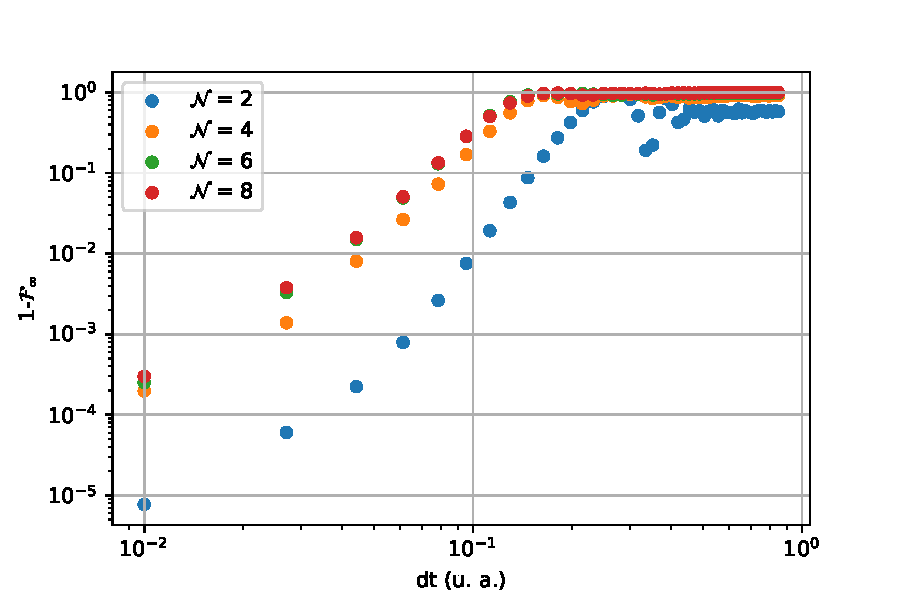
\includegraphics[scale=0.8]{longTimeFloquetFidelity.pdf}
      \caption{Long time state infidelity as a function of integration time step $\Delta t$. Different sets of data are taken for system sizes $\mathcal{N} = 2,4,6,8$. Units are normalized to $\hbar = 1$. This normalization is denoted $(u. a.)$.}
      \label{fig:FloquetDynamics}
    \end{figure}

\section{Circuit implementations}
\label{sec:MainCircuits}
  
  On chapter \ref{chap:qc}, some networks for simulating time evolution of the two-qubit Hamiltonian were introduced (see fig. \ref{fig:salathe-includes}). In this section, three possible transpiled circuits are introduced. Those implement the single qubit and two qubit operators on equation \ref{eq:HamiltonianDecomposition}. The single qubit operators are implemented in the same way on all three alternatives. Each circuit differs from the others on the implementation of the two spin operators. The first alternative is a direct basis transpilation, based on the controlled phase gate. The second alternative is one that takes advantage of the commutation properties of the local two spin Hamiltonian. This alternative was derived mostly independently from \cite{BellUniversalCartan} at early stages of the present work. However, a thorough discussion of the insights required to derive this circuit is included. The last option is a cross resonance based implementation, as discussed on chapter \ref{chap:qc}.

  \subsection{Simulation of field interaction}
  \label{subsec:fieldInteractionCircuit}

    To simulate evolution under Hamiltonian \ref{eq:HamiltonianDecomposition}, a direct approach would be to us te definition of single qubit rotations, and implement a second order trotterization scheme as illustrated on figure \ref{fig:directSimulationFieldSpin}. However, exact simulation of this model is possible by rotating the Bloch sphere main axes so that the external field points to the $\hat{z}$ direction. This can be done by the operator

    \begin{equation}
      \hat{U}_{\theta,\phi} = \begin{bmatrix}
        \cos(\frac{\theta}{2}) & \sin(\frac{\theta}{2}) \\
        \mathrm{e}^{\mathrm{i}\phi}\sin(\frac{\theta}{2}) & -\mathrm{e}^{\mathrm{i}\phi}\cos(\frac{\theta}{2}),
      \end{bmatrix}
      \label{eq:UGate}
    \end{equation}

    \noindent where $\theta$ and $\phi$ are defined by the spherical representation of the external field (see eq. \ref{eq:PolarRepresentation}):

    \begin{gather}
      h^2 =  (h_i^{(x)})^2 + (h_i^{(y)})^2 + (h_i^{(z)})^2 ,\\
      h_i^{(x)} = h \sin(\theta)\cos(\phi), \\
      h_i^{(y)} = h \sin(\theta)\sin(\phi), \\
      h_i^{(z)} = h \cos(\theta).
      \label{eq:PolarRepresentation}
    \end{gather}

    This approach is illustrated on figure \ref{fig:rotatedSimulationFieldSpin}. Therefore, at the same computational cost, this interaction can be simulated exactly by the former algorithm.

    \begin{figure}
    \centering
    \begin{subfigure}[b]{1.0\textwidth}
        \centering
        \caption{}
        \begin{quantikz}
            & \gate{\hat{R}_{\hat{x},2h_i^{(X)}\Delta t}} & \gate{\hat{R}_{\hat{y},2h_i^{(Y)}\Delta t}} & \gate{\hat{R}_{\hat{z},2h_i^{(Z)}\Delta t}} & \qw
        \end{quantikz}
        \label{fig:directSimulationFieldSpin}
    \end{subfigure}
    \begin{subfigure}[b]{1.0\textwidth}
        \centering
        \caption{}
        \begin{quantikz}
            & \gate{\hat{U}_{\theta,\phi}^{\dagger}} & \gate{\hat{R}_{\hat{z},2h \Delta t}} & \gate{\hat{U}_{\theta,\phi}} & \qw
        \end{quantikz}
        \label{fig:rotatedSimulationFieldSpin}
    \end{subfigure}
    \caption{(a) Direct trotterization of field-spin interaction for small time interval $\Delta t$. (b) Exact simulation by rotating the Bloch sphere reference frame to the external field direction.}
    \label{fig:directTrotterizationFieldSpin}
\end{figure}

  \subsection{Simulation of Two-spin Interaction}
  \label{subsec:TwoSpinCircuits}

    The simpler spin-spin Hamiltonian

    \begin{equation}
      \hat{H}_{ij} = J_{ij}^{(X)} \hat{X}_i \hat{X}_j + J_{ij}^{(Y)} \hat{Y}_i \hat{Y}_j + J_{ij}^{(Z)} \hat{Z}_i \hat{Z}_j
      \label{eq:SpinSpin}
    \end{equation}

    \noindent is simulated using IBM Quantum device's universal set, or cross resonance pulses. This is the most computationally expensive part of the evolution scheme. As may be seen on figure \ref{fig:echoedPulseQiskit}, the most time consuming processes are simulating two qubit interactions. In consequence, reducing the number and duration of CNOT gates or cross resonance pulses on the evolution algorithm is crucial for obtaining high fidelity results. Here, a first network that performs direct transpilation of circuit \ref{fig:heras-hubbard} is presented. It will be used as a control case, since non-optimized transpilations would yield this network for simulating the Hamiltonian \cite{Qiskit}. A basis efficient circuit is introduced, and its mathematical and physical insights are discussed \cite{BellUniversalCartan}. Finally, the pulse efficient network proposed on \cite{RXZPulseEfficient} is revisited.
    
    \subsubsection{Direct transpilation circuit}
    \label{subsubsec:DirectTranspilationCircuit}

      To adapt circuit \ref{fig:heras-hubbard} for IBM Quantum devices, it is helpful to note that

      \begin{equation}
        \mathrm{e}^{-\mathrm{i}\phi \hat{Z}_i \otimes \hat{Z}_j} = \cos(\frac{\phi}{2}) - \mathrm{i}\sin(\frac{\phi}{2}) \hat{Z}_i \otimes \hat{Z}_j = 
        \begin{bmatrix}
          \mathrm{e}^{-\mathrm{i}\frac{\phi}{2}} & 0 & 0 & 0 \\
          0 & \mathrm{e}^{\mathrm{i}\frac{\phi}{2}} & 0 & 0 \\
          0 & 0 & \mathrm{e}^{\mathrm{i}\frac{\phi}{2}} & 0 \\
          0 & 0 & 0 & \mathrm{e}^{-\mathrm{i}\frac{\phi}{2}}.
        \end{bmatrix}
        \label{eq:expZZ}
      \end{equation}

      By the definition of CNOT gate, and single-qubit gates (see chap. \ref{chap:qc}), it follows that this operator can be implemented by the circuit on figure \ref{fig:directTrotterSpinZZ}. A direct way to simulate the $XX$ interaction term is to note that

      \begin{equation}
        \hat{H}^{\otimes 2} \mathrm{e}^{-\mathrm{i}\phi \hat{Z}_i \otimes \hat{Z}_j} \hat{H}^{\otimes 2} = \mathrm{e}^{-\mathrm{i}\phi \hat{X}_i \otimes \hat{X}_j},
        \label{eq:Z2X}
      \end{equation}

      \noindent where $\hat{H}$ means the Hadamard gate, not the target Hamiltonian. This follows from the observation that $\hat{H}\hat{Z}\hat{H} = \hat{X}$. In a similar fashion, it is possible to implement the $YY$ interaction by noticing that

      \begin{equation}
        \Big(\hat{R}_{\hat{z}, \pi/2}^{\dagger}\hat{H}\Big)\hat{Z}\Big(\hat{R}_{\hat{z}, \pi/2}^{\dagger}\hat{H}\Big)^{\dagger} = \hat{Y}.
        \label{eq:Z2Y}
      \end{equation}

      \begin{figure}
    \centering
    \begin{subfigure}[b]{1.0\textwidth}
        \centering
        \caption{}
        \begin{quantikz}
            & \ctrl{1} & \qw & \ctrl{1} & \qw \\
            & \targ{}  & \gate{\hat{R}_{\hat{z}, \phi}} & \targ{} & \qw\\
        \end{quantikz}
        \label{fig:directTrotterSpinZZ}
    \end{subfigure}
    \begin{subfigure}[b]{1.0\textwidth}
        \centering
        \caption{}
        \begin{quantikz}
            & \gate{H} & \ctrl{1} & \qw & \ctrl{1} & \gate{H} & \qw \\
            & \gate{H} & \targ{}  & \gate{\hat{R}_{\hat{z}, \phi}} & \targ{} & \gate{H}& \qw\\
        \end{quantikz}
        \label{fig:directTrotterSpinXX}
    \end{subfigure}
    \begin{subfigure}[b]{1.0\textwidth}
        \centering
        \caption{}
        \begin{quantikz}
            & \gate{\hat{R}_{\hat{z}, \pi/2}^{\dagger}} & \gate{H} & \ctrl{1} & \qw & \ctrl{1} & \gate{H} & \gate{\hat{R}_{\hat{z}, \pi/2}} & \qw \\
            & \gate{\hat{R}_{\hat{z}, \pi/2}^{\dagger}} & \gate{H} & \targ{}  & \gate{\hat{R}_{\hat{z}, \phi}} & \targ{} & \gate{H} & \gate{\hat{R}_{\hat{z}, \pi/2}} & \qw\\
        \end{quantikz}
        \label{fig:directTrotterSpinYY}
    \end{subfigure}
    \caption{(a) Implementation of two-spin $ZZ$ interaction using IBM Quantum's universal set. (b) Implementation of $XX$ interaction using basis rotation. (c) Implementation of $YY$ interaction using the same technique as in (b).}
    \label{fig:directTrotterSpinSpin}
\end{figure}

      This leads to a straightforward algorithm for simulating spin-spin interaction that uses 6 CNOT gates, and 15 single-qubit rotations. 
    
    \subsubsection{Basis efficient circuit}
    \label{subsubsec:BasisEfficientCircuit}

      This gate count can be reduced further by considering the commutation relations between the operators that constitute the spin-spin interaction Hamiltonian

      \begin{equation}
        [\hat{X}_i\hat{X}_j, \hat{Z}_i\hat{Z}_j] = [\hat{Y}_i\hat{Y}_j, \hat{Z}_i\hat{Z}_j] = 0.
        \label{eq:CommutationRelations}
      \end{equation}

      From basic quantum mechanics, there exists a basis that diagonalizes Hamiltonian \ref{eq:SpinSpin}. By an appropriate rotation, evolution can be performed using mostly $\hat{z}$ axis rotations, and few two-qubit operations. This basis is straightforward to find by noticing that the \textit{total spin} operator

      \begin{equation}
        \hat{S}^2 = 6 + 2\Big(\hat{X}_i\hat{X}_j + \hat{Y}_i\hat{Z}_j + \hat{Z}_j\Big) 
        \label{eq:TotalSpin}
      \end{equation}

      \noindent commutes with the spin-spin interaction Hamiltonian. From elementary quantum physics, it is known that the eigenstates of such operator are the singlet and triplet states \cite{Beck}. By mapping quantum bit value to spin value directly, it can be readily seen that the singlet and triplet states correspond exactly to the \textit{Bell states} defined on equations \ref{eq:BellBasis}. By considering that

      \begin{gather}
        \hat{X}_i\hat{X}_j \ket{\Phi^{\pm}} = \pm\ket{\Phi^{\pm}}, \\
        \hat{Y}_i\hat{Y}_j \ket{\Phi^{\pm}} = \mp\ket{\Phi^{\pm}}, \\
        \hat{Z}_i\hat{Z}_j \ket{\Phi^{\pm}} = \ket{\Phi^{\pm}},
        \label{eq:PhiBellBasisOps}
      \end{gather}

      \begin{gather}
        \hat{X}_i\hat{X}_j \ket{\Psi^{\pm}} = \pm\ket{\Psi^{\pm}}, \\
        \hat{Y}_i\hat{Y}_j \ket{\Psi^{\pm}} = \pm\ket{\Psi^{\pm}}, \\
        \hat{Z}_i\hat{Z}_j \ket{\Psi^{\pm}} = -\ket{\Psi^{\pm}},
        \label{eq:PsiBellBasisOps}
      \end{gather}

      \noindent it is possible to obtain the energies of the Hamiltonian:

      \begin{gather}
        \hat{H}_{ij} \ket{\Psi^{\pm}} = \bigg(-J_{ij}^{(Z)} \pm (J_{ij}^{(X)} + J_{ij}^{(Y)})\bigg) \ket{\Psi^{\pm}}, \\
        \hat{H}_{ij} \ket{\Phi^{\pm}} = \bigg(J_{ij}^{(Z)} \pm (J_{ij}^{(X)} - J_{ij}^{(Y)})\bigg) \ket{\Phi^{\pm}}.
        \label{eq:SpinSpinEnergies}
      \end{gather}

      Define phases

      \begin{gather}
        \phi_{xx} = 2 J_{ij}^{(X)} \Delta t, \\
        \phi_{yy} = -2 J_{ij}^{(Y)} \Delta t, \\
        \phi_{zz} = 2 J_{ij}^{(Z)} \Delta t,
        \label{eq:SpinSpinPhases}
      \end{gather}
      
      \noindent where $\Delta t$ is the time interval to be simulated. A quantum circuit representing this approach to evolution is presented on figure \ref{fig:abelianTrotterSpinSpin}. Main stages are separated by slices, which correspond to:

      \begin{enumerate}
        \item Basis change from computational to Bell.
        \item Append $\phi_{xx}$ and $\phi_{zz}$ phases.
        \item Shuffle the basis to append $\phi_{yy}$ phase.
        \item Return to ordered Bell basis
      \end{enumerate}

      In the first stage, the Bell basis is mapped according to

      \begin{gather}
        \ket{\Phi^{+}} \rightarrow \ket{00}, \\
        \ket{\Phi^{-}} \rightarrow \ket{01}, \\
        \ket{\Psi^{+}} \rightarrow \ket{10}, \\
        \ket{\Psi^{-}} \rightarrow \ket{11}. 
      \end{gather}

      From equations \ref{eq:SpinSpinEnergies}, it may be noted that $xx$ phase correlates to the less significant bit, while $zz$ phase correlates to the most significant bit. Also, $yy$ phase correlates to the parity of the mapped computational basis state, hence the need of a CNOT gate. The last part undoes the CNOT gate action on the previous step, and returns to the Bell basis. The direct way to perform the last step is illustrated on figure \ref{fig:abelianTrotterSpinSpin}(a). A more clever approach relies on the following equalities (up to global state phases)

      \begin{gather}
        \ket{\Phi^{+}} = \frac{1}{\sqrt{2}}(\ket{00} + \ket{11}) = \frac{1}{\sqrt{2}}(\ket{+\mathrm{i},-\mathrm{i}} + \ket{-\mathrm{i},+\mathrm{i}}), \\
        \ket{\Phi^{-}} = \frac{1}{\sqrt{2}}(\ket{00} - \ket{11}) = \frac{1}{\sqrt{2}}(\ket{+\mathrm{i},+\mathrm{i}} + \ket{-\mathrm{i},-\mathrm{i}}), \\
        \ket{\Psi^{+}} = \frac{1}{\sqrt{2}}(\ket{01} + \ket{10}) = \frac{1}{\sqrt{2}}(\ket{+\mathrm{i},+\mathrm{i}} - \ket{-\mathrm{i},-\mathrm{i}}), \\
        \ket{\Psi^{-}} = \frac{1}{\sqrt{2}}(\ket{01} - \ket{10}) = \frac{1}{\sqrt{2}}(\ket{+\mathrm{i},-\mathrm{i}} - \ket{-\mathrm{i},+\mathrm{i}}), 
        \label{eq:bellOnYBasis}
      \end{gather}

      \noindent where the single qubit states $\{\ket{+\mathrm{i}}, \ket{+\mathrm{i}}\}$ are defined as on chapter \ref{chap:qc}, and correspond to the $\hat{Y}$ eigenstates. The shuffling stage that appends $yy$ phase actually permutes states $\ket{\Psi^{-}}$ and $\ket{\Psi^{+}}$ of the Bell basis. It is now easy to see that by performing single qubit rotations that are equivalent to the mappings (where the subindex corresponds to qubits 0 and 1, respectively)

      \begin{gather}
        \ket{0}_0 \rightarrow \ket{-\mathrm{i}}_0, \\
        \ket{1}_0 \rightarrow -\mathrm{i}\ket{+\mathrm{i}}_0, \\
        \ket{0}_1 \rightarrow \ket{+\mathrm{i}}_1, \\
        \ket{1}_1 \rightarrow \mathrm{i}\ket{-\mathrm{i}}_1, \\
        \label{eq:localBellShuffling}
      \end{gather}

       \noindent it is possible to perform the desired reordering without using an additional CNOT gate. Such procedure is illustrated on figure \ref{fig:abelianTrotterSpinSpin}(b). On the last state, the computational basis is mapped back to the Bell basis, and the reordering is performed on the Bell basis using local rotations that correspond to transformation \ref{eq:localBellShuffling}. As a result, the number of expensive CNOT gates has been halved with respect to the direct transpilation circuit.

      \begin{figure}
    \centering
    \begin{quantikz}
        & \ctrl{1} & \gate{H} & \gate{\hat{R}_{\hat{z}, \phi_{xx}}} & \ctrl{1}  & \qw                                 & \ctrl{1} & \gate{H} & \ctrl{1} & \qw \\
        & \targ{}  & \qw      & \gate{\hat{R}_{\hat{z}, \phi_{zz}}} & \targ{}  & \gate{\hat{R}_{\hat{z}, \phi_{yy}}} & \targ{}  & \qw      & \targ{}  & \qw \\
    \end{quantikz}
    \caption{Implementation of spin-spin interaction using abelian groups. The first and last two stages perform a change of basis to Bell basis from computational basis. Interaction phases are appended according to the energy values (see eq. \ref{eq:SpinSpinPhases}).}
    \label{fig:abelianTrotterSpinSpin}
\end{figure}

    \subsection{Pulse efficient implementation}
    \label{subsubsec:PulseEfficientCircuit}

      On subsection \ref{subsec:EchoedCrossResonance}, a pulse schedule, introduced in \cite{RXZPulseEfficient}, was presented as an efficient alternative for implementing the unitary operators

      \begin{equation}
        \hat{U}(\alpha, \beta, \gamma) = \mathrm{e}^{-\mathrm{i}(\alpha\hat{X}\hat{X} + \beta\hat{Y}\hat{Y} + \gamma\hat{Z}\hat{Z})}
        \label{eq:CartanDecomp2}.
      \end{equation}

      It can be readily seen that the relations

      \begin{gather}
        \alpha = J_{xx} \Delta t, \\
        \beta = J_{yy} \Delta t, \\
        \gamma = J_{zz} \Delta t,
      \end{gather}

      \noindent yield a unitary that exactly performs time evolution under the two-spin interaction Hamiltonian. The single qubit rotations used on the network representation \ref{fig:PulseEffcientCartanCircuit} profit from the relations between Pauli operators stated on equations \ref{eq:Z2X} and \ref{eq:Z2Y}. This algorithm has a slightly different nature than those presented previously. The former two use a particular basis to implement a quantum algorithm that can run on any universal device, regardless of the underlying architecture. The one discussed here, on the other hand, is specifically calibrated for IBM Quantum devices using Qiskit SDK and the pulse scaling technique implemented on \cite{RXZPulseEfficient}.

\section{Comparison and Benchmark: Methodology}
\label{sec:Methodology}

  In general, time simulation of a quantum system has at least two requirements: 1) that the state after evolution resembles within given error bounds the actual target state, and 2) that expected values of interesting observables can be extracted within given error bounds. In the present work, those two requirements are assessed by considering expected value time evolution, probability density (pdf) time evolution, and target probability density fidelity. In this section, the fundamental methods for implementing experiments on quantum devices, measuring observables and computing simulation fidelities are discussed. A benchmark system with Hamiltonian

  \begin{equation}
    \hat{H} = \sum_{i=0}^{1}\Bigg(\hat{X}_i\hat{X}_{i+1} + \hat{Y}_i\hat{Y}_{i+1} + \hat{Z}_i\hat{Z}_{i+1} \Bigg)
    \label{eq:BenchmarkHamiltonian}
  \end{equation}

  \noindent is used for simulation on \textit{ibmq jakarta}. The three proposed schemes discussed on previous sections will be benchmarked by computing the metric mentioned above, for this particular system \footnote{In principle, a larger system could be simulated. However, direct pulse control using the methods proposed on \cite{RXZPulseEfficient} depends on the connectivity if quantum devices. \textit{ibmq jakarta} only supports this type of control on a set of three qubits. Hence the constraints for comparison between the propsed algorithms.}. As a control case, a Qiskit's QASM simulator is used to perform time evolution, since it emulates fault-tolerant quantum computation. This base case will be used for comparing the results obtained by performing the experiment on actual quantum devices and further analysis and discussion.

  \subsection{Measurement of observables}
  \label{subsec:MeasurementMethods}

    Consider the set of of Pauli tensor product operators defined on a space of $N$ qubits. Each of this operators can be mapped to the set of strings whose characters indicate the Pauli operator that acts on the corresponding qubit. For instance,

    \begin{equation}
      \hat{I} \otimes \hat{X} \otimes \hat{X},
    \end{equation}

    \noindent denotes a Pauli string operator that acts on a 3-qubit space, and applies and identity gate on the third qubit, while applying an $X$ gate on the first two. It is a well known fact that the set of Pauli tensor product operators constitute a basis for the space of operators defined on an $N$-qubit system's Hilbert space \cite{Nielsen, Strini}. Hence, any operator in that space has the expansion
    
    \begin{equation}
      \hat{O} = \sum_{P} c_P \hat{P}
    \end{equation}

    \noindent where $P$ is a Pauli tensor product operator. This fact yields a direct approach towards measuring expected value of operators. If the expected value of Pauli tensors can be measured, then linearity yields the expected value of any $N$-qubit operator. Now, by default, experiments performed on IBM's quantum devices produce the expected value of the Pauli tensor $\otimes^{N} \hat{Z}$. As a result, by applying local rotations to the qubits according to equations \ref{eq:Z2X} and \ref{eq:Z2Y}, it is possible to measure any Pauli tensor that also includes $\hat{X}$ and $\hat{Y}$ operators. It might be the case that the measured Pauli tensor only acts on a subspace of the register. This is irrelevant, though, since it is possible to trace out the measured subsystem, thus making any action on the complementary system irrelevant \cite{Nielsen}. Hence, measuring all the qubits of the register at once, on each experiment, and applying local rotations, is a valid methodology for recovering any pdf.

    Measuring the probability density is quite straightforward using Qiskit SDK. As mentioned before, the results of the execution of most quantum algorithms produce a single outcome of measuring the register on the computational basis, which can be mapped to a binary string. Approximate reconstruction of the pdf can be carried out by repeating the experiment several times and building an histogram. This is done by Qiskit methods. Once the pdf is reconstructed, the expected value of the operator $\otimes^{N} \hat{Z}$ can be reconstructed by examining the parity of the outcome string, i.e., by the formula
    
    \begin{equation}
      \expval{\otimes^{N} \hat{Z}} = \sum_{s \in \{0,1\}^{N}\}} p(s) \prod_{i \in s} (-1)^{i},
      \label{eq:expValPauliZ}
    \end{equation}

    \noindent where $p(s)$ denots the probability density of the outcomes, and $(-1)^{i}$ is the parity of the characters in the string. By applying local rotations, it is possible to rotate any state from the eigenbasis of any Pauli tensor operator to the computational basis. As a result, the procedure yields the expected value of any Pauli tensor. Linearity does the rest.

    \subsubsection{Readout Error Correction}
    \label{subsubsec:readoutErrorCorrection}

      It must be noted that actual quantum device experience readout errors after measurement. This readout errors are typically modeled like random bit flip channels \cite{Nielsen, Strini}. Suppose that prior to measurement, a quantum state has an associated pdf $p_i$ of measurement on the computational basis. Due to bit flip noise, the actual measured probability is

      \begin{equation}
        p_i' = M_{ij} p_j,
        \label{eq:MarkovMatrix}
      \end{equation}

      \noindent where $M_{ij}$ is the \textit{transition matrix} of the process. To correct readout errors, the transition matrix is measured by preparing the states of the computational basis and performing several measurements in order to get an approximate noisy pdf. Then, the corrected pdf is obtained by inverting the transition matrix as follows:

      \begin{equation}
        p_i = M_{ij}^{-1} p_j'.
        \label{eq:MarkovMatrix}
      \end{equation}

      This procedure is applied any time a pdf is computed from a series of experiments on actual quantum devices. The predefined Qiskit interfaces for this task is used on the implementations.

    \subsubsection{Measuring probability density fidelity}
    \label{subsubsec:PdfFidelityMeasurement}

      In this work, probability density fidelity is used as a quantitative measure of the precision of the evolution. Consider two states $\ket{\psi}$ and $\ket{\psi'}$, that yield two probability densities of measurement in the computational basis, $p_i$ and $p_i'$, respectively. The probability density fidelity of those two distributions is defined \cite{HubbardSimulLasHeras} by the equation

      \begin{equation}
        F_{p_i, p_i'} = \big(\sum_i \sqrt{p_i p_i'}\big)^2.
        \label{eq:PdfFidelityDefinition}
      \end{equation}

      To assess the precision of a time evolution scheme, a target evolution time is fixed, as well as a fixed number of integration steps. The initial state

      \begin{equation}
        \ket{\psi} = \ket{110}
        \label{eq:initialStateBenchmark}
      \end{equation}

      \noindent is evolved using the evolution scheme (by running experiments on \textit{ibmq jakarta}), thus yielding a pdf ($p_i'$) as described in this subsection. The exact pdf ($p_i$) is computed by exact time evolution using numerical diagonalization of the Hamiltonian. The probability density fidelity, for given time and number of integration steps is computed according to equation \ref{eq:PdfFidelityDefinition}.

  \subsection{Device specifications}
  \label{subsec:ibmq_jakartaSpecs}

    All experiments are run on \textit{ibmq jakarta}, a backend with a processor Falcon r5.1H, at the time of development of this work. This processor has seven physical qubits. It has a connectivity as depicted on figure \ref{fig:JakartaConnectivity}. It supports pulse control as on \cite{RXZPulseEfficient}, only on qubits 1, 3, and 5. Like all IBM Quantum devices, its basis set is $\{\hat{S}_x = \sqrt{\hat{X}}, \hat{X}, \hat{R}_{z,\phi} \}$. Those are logical gates, and most of the time, actual execution requires performing swap operations between some qubits due to limited connectivity.

    \begin{figure}
      \centering
      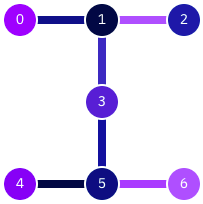
\includegraphics[scale=0.6]{ibmqJakarta.png}
      \caption{Connectivity of \textit{ibmq jakarta} processor. Taken from the official IBM Quantum site.}
      \label{fig:JakartaConnectivity}
    \end{figure}

    Experiments involving direct transpilation and gate-efficient schemes, are performed using qubits 0, 1, and 2. While experiments involving pulse-efficient schemes are performed on qubits 1, 3, and 5. Quantum devices are calibrated each day, and may vary. However, typical parameter values are reported on table \ref{tab:jakartaParams}.

    \begin{table}[!htbp]
      \begin{center}
        \begin{tabular}{| c | c |}
          \hline 
          $T_1$ & 130 $\mu$s \\
          \hline
          $T_2$ & 34 $\mu$s \\
          \hline
          $\epsilon_{\text{CNOT}}$ & 1\% \\
          \hline
          $\epsilon_{\text{Read}}$ & 2\% \\
          \hline
        \end{tabular}
      \end{center}
      \caption{Typical parameter values for \textit{ibmq jakarta}. The coherence times are discussed on the previous chapter. $\epsilon_O$ denotes the error on performing an operation $O$. In this case, CNOT gates and readout.}
      \label{tab:jakartaParams}
    \end{table}
  
    \begin{table}[!htbp]
      \begin{center}
        \begin{tabular}{| c | c |}
          \hline 
          $0 \rightarrow 1$ & 234.7 ns \\
          \hline
          $1 \rightarrow 2$ & 288.4 ns \\
          \hline
          $1 \rightarrow 3$ & 384.0 ns \\
          \hline
          $3 \rightarrow 5$ & 341.3 ns \\
          \hline
          $4 \rightarrow 5$ & 405.3 ns \\
          \hline
          $5 \rightarrow 6$ & 312.9 ns \\
          \hline
        \end{tabular}
      \end{center}
      \caption{Execution times of CNOT gates on \textit{ibmq jakarta}. The column on the left denotes control-target pairs, and the right, the execution time in nanoseconds. Times were acquired using Qiskit API, and is reported from the backend calibration data.}
      \label{tab:jakartaCnotTimes}
    \end{table}

  \subsection{Control case: QASM Simulation Results}
  \label{subsec:QASMResults}

    To establish a control case for evaluating results of quantum evolution on real devices, the benchmark system is simulated over a time $t = 1$ using an integration step $dt = 1/8$. In a more quantitative test, the probability density fidelity is computed for times $t = 1, 2, 3$, with up to $8$ integration steps. Units of time are normalized to $\hbar = 1$, so that energy has units of inverse time. These results represent the outcome of executing the direct evolution scheme introduced on section \ref{sec:MainCircuits}, on a fault tolerant device. In figures \ref{fig:QASMpdf} and \ref{fig:QASMpaulis}, the results of evolution with direct diagonalization of the Hamiltonian are presented as dotted lines.

    Probability density of measuring a 3-bit string is evolved over time. The convention is that the string is represented by its associated number in decimal system. Expected values of single qubit Pauli operators $\hat{X}_i, \hat{Y}_i, \hat{Z}_i$ are measured for each of the qubits. The first qubit observables correspond to color red data, the second qubit's, to blue data, and the third qubit's, to black data. This convention holds on all graphics of this type. Probability density fidelity is computed for several number of integration steps $N$ (up to eight), and each point correspond to the average of five sets of 2048 experimental repetitions.

    A small number of integration steps is used since the finite coherence times of the qubits in the device limit the depth of the circuit that can be executed on real devices. If the gate execution times approach the coherence times, the state coherence is irreversibly lost, and thus the final state does not resemble at all the target final state. As may be seen on figure \ref{fig:QASMfidelity}, there is a sort of transient stage during which the Trotter approximation does not converge. As seen before, there exists a critical integration time step $\Delta t$, below which the state fidelity has a predictable approximation error. It may be also noted that high fidelities can be achieved by using a relatively small number of integration steps. Furthermore, observables resemble quite well the theoretical values. This indicates that as long as the integration time step $\Delta t = t / N$ is below the convergence threshold, the trotter error can be controlled.

    \begin{figure}
      \thisfloatpagestyle{empty}
      \centering
      \begin{subfigure}[b]{1.0\textwidth}
        \centering
        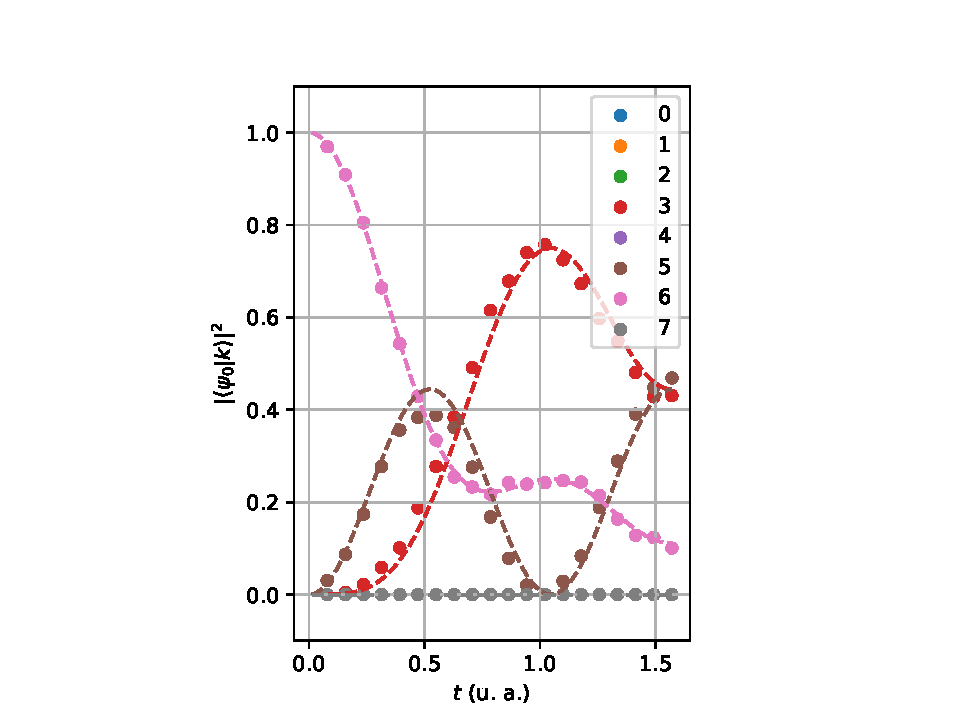
\includegraphics[scale=0.65]{QASMData/qasm_control_pdf_evol.pdf}
        \caption{Time evolution of probability density (pdf) of the benchmark system initialized on the state $\ket{\psi_0} = \ket{110}$, for a time $t=1$. The numbers in the convention are those whose binary representation corresponds to $\ket{k}$.}
        \label{fig:QASMpdf}
      \end{subfigure}
      \hfill
      \begin{subfigure}[b]{1.0\textwidth}
        \centering
        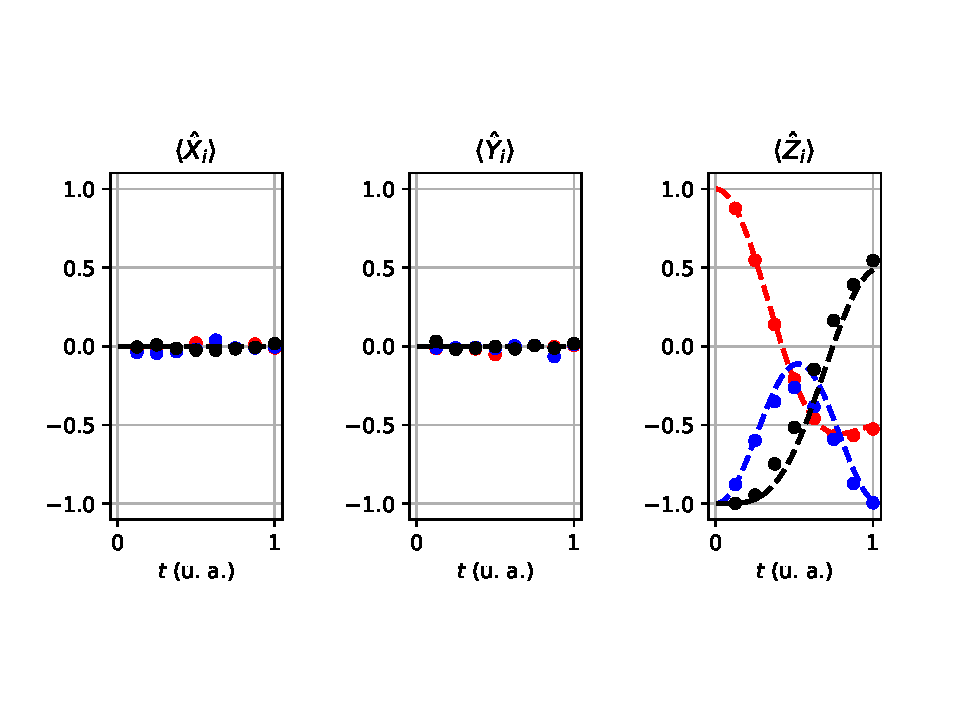
\includegraphics[scale=0.65, trim={0 1.8cm 0 1.8cm}, clip]{QASMData/qasm_control_pauli_exps.pdf}
        \caption{Time evolution of single qubit Pauli operators of the benchmark system initialized on the state $\ket{110}$, for a time $t=1$. The first qubit observables correspond to color red data, the second qubit's, to blue data, and the third qubit's, to black data}
        \label{fig:QASMpaulis}
      \end{subfigure}
      \begin{subfigure}[b]{1.0\textwidth}
        \centering
        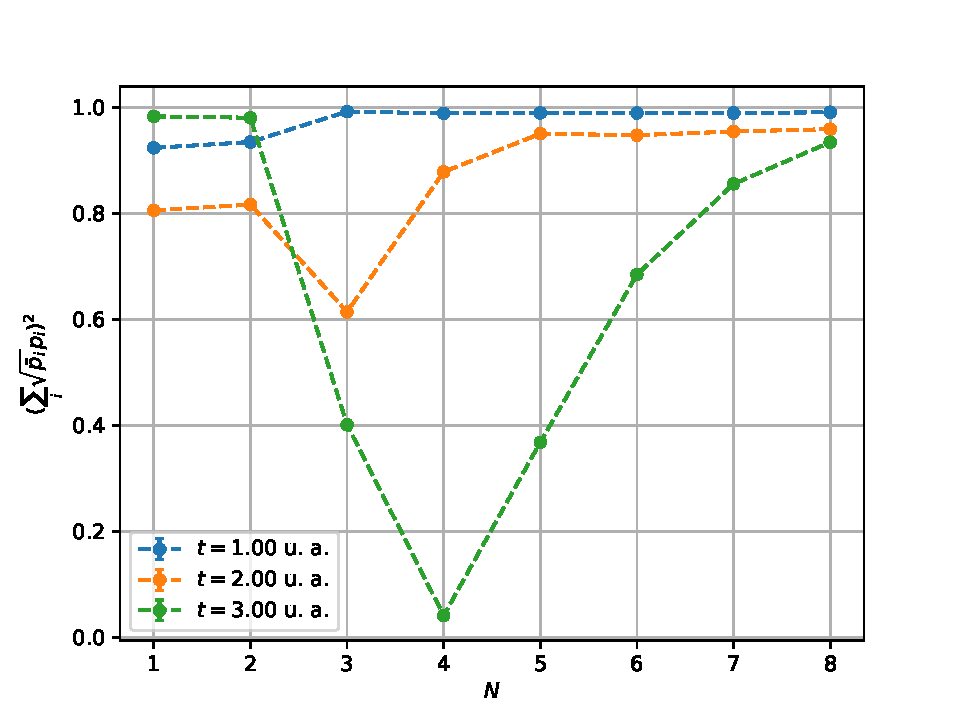
\includegraphics[scale=0.65]{QASMData/qasm_control_pdf_fidelity.pdf}
        \caption{Probability density fidelity as a function of the number of integration steps, $N$, and simulation times $t = 1, 2, 3$. Each point corresponds to the average of five sets of experiments. Notice that the transient behavior mentioned lasts up to about $N = 4$.}
        \label{fig:QASMfidelity}
      \end{subfigure}
      \caption{QASM Simulation results. Time units are normalized to $\hbar=1$ and $J_{ij}^{(X)} = J_{ij}^{(Y)} = J_{ij}^{(Z)} = 1$}. This is denoted by (u. a.).
      \label{fig:QASMResults}
    \end{figure}

\section{Comparison and Benchmark: Results}
\label{sec:Results}

    Now that the main metrics, and the way they are measured using \textit{ibmq jakarta}, results of simulation using the schemes proposed on section \ref{sec:MainCircuits} are presented. Results are compared to fault-tolerant simulation outcome in figure \ref{fig:QASMResults}.

    Expected values of single qubit observables are measured following conventions established on section \ref{subsec:QASMResults}. From figure \ref{fig:PauliExpectedValues}, it can be seen that the scheme that produces the largest resemblance to the ideal values (dotted lines) is the pulse efficient implementation, followed by the basis efficient and the direct transpilation. Qualitatively, the difference in performance is overwhelming. While the base efficient and direct transpilation approaches struggle to converge for four steps, the pulse efficient scheme is able to converge surprisingly well for the entire set of eight steps. Since the calibration of entangling gates is the same for all cases (except for a parameter scaling on pulse efficient experiments) it can be inferred that the use of shorter entangling pulses, which improves the usage of the finite coherence times of the system, is the most determinant factor when simulating this kind of Hamiltonians.

    Those features can be seen more clearly on figure \ref{fig:PdfExpectedValues}. From the ideal results on figure \ref{fig:QASMResults}, it can be seen that the probability density only presents oscillations for states $\ket{3}$, $\ket{6}$, and $\ket{5}$. Figures \ref{fig:PdfDirectTransp} and \ref{fig:PdfBasis} suggest that the state coherence is lost very fast (qubits depolarize fairly quickly), and the probability density fidelity decays very rapidly as the circuit depth of simulation increases, using both direct and basis efficient schemes. On the other hand, pulse efficient schemes seem to better maintain state coherence since the execution time of each trotter step is shorter. As a result, the state fidelity is larger.

    On figure \ref{fig:PdfExpectedFidelity}, these observations are made more quantitative. After the transient stage in which the Trotter approximation does not converge in general, it can be seen that the probability density fidelity decays consistently for direct transpilation and basis efficient schemes, as the number of integration steps increase. On the other hand, pulse efficient schemes have an increasing fidelity with the number of integration steps. While the first two schemes produce fidelities near 30\% - 40\%, direct pulse control yields fidelities near 70\% in some cases, having actual execution times about 40\% shorter. There is a caveat, though. As the integration time step increases, the benefits of pulse schemes is reduced, since the actual execution time increases proportionally (see figure \ref{fig:PulseDurationVdt}). This can be seen on figure \ref{fig:PdfPulseFidelity}. As the target simulation time increases, the fidelity remains below 50\%. Since the circuit depth does not change with respect to shorter times, it can be concluded that this reduction in the fidelity is due to the larger execution time of the experiments (see figure \ref{fig:PulseDurationVdt}). In consequence, simulating anisotropic Heisenberg Hamiltonians on quantum computers imply optimizing the tradeoff between short Trotter steps with pulse control, and a large number of repetitions required to simulate large times. As may be inferred from figure \ref{fig:FloquetDynamics}, it must be procured that the integration time step $\Delta t$ is below the threshold for predictable Trotter error control, though.

    \begin{figure}
      \centering
      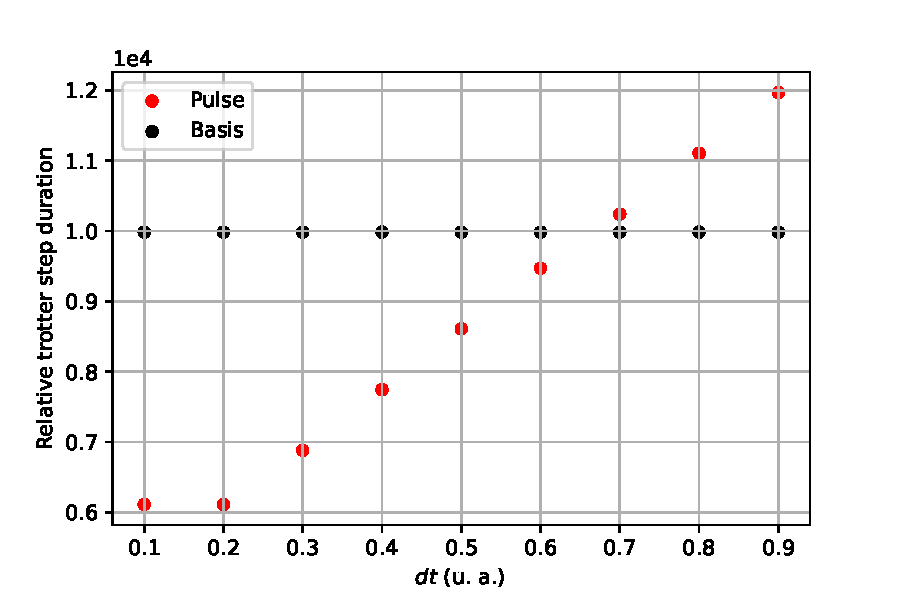
\includegraphics[scale=0.72]{schedTimeDurationPlot.pdf}
      \caption{Execution time (in relative units) of pulse efficient and basis efficient Trotter steps on IBM Quantum devices as a function of integration time step $\Delta t$.}
      \label{fig:PulseDurationVdt}
    \end{figure}

    \begin{figure}
      \centering
      \begin{subfigure}[b]{1.0 \textwidth}
        \centering
        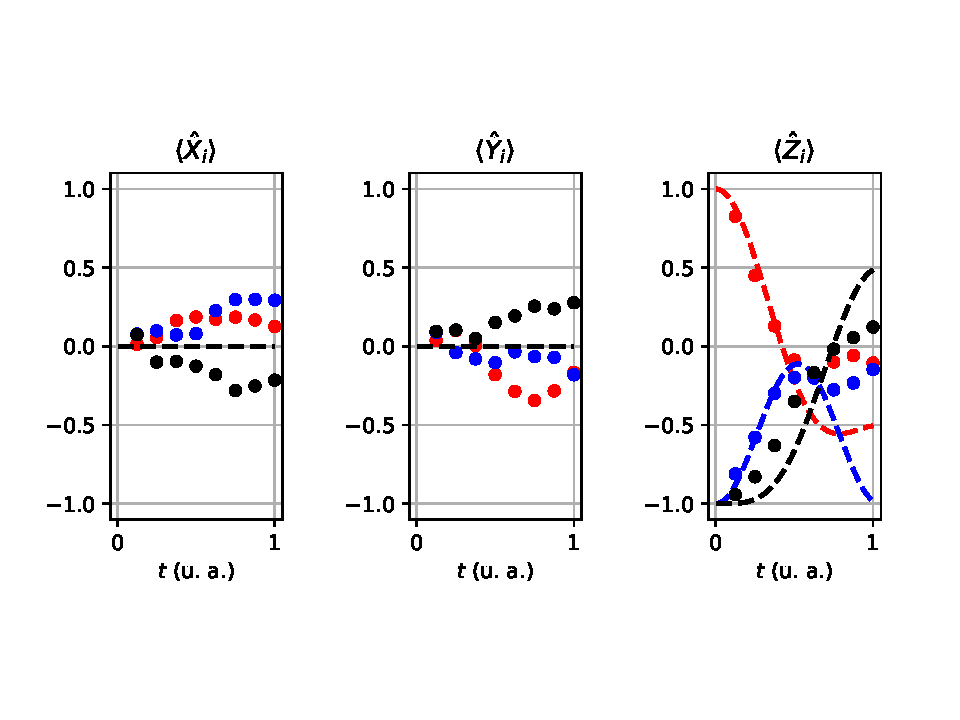
\includegraphics[scale=0.8, trim={0 1.8cm 0 1.8cm}, clip]{DirectTranspilationData/direct_pauli_exps.pdf}
        \caption{Direct transpilation expected values}
        \label{fig:PauliDirectTransp}
      \end{subfigure}
      \begin{subfigure}[b]{1.0 \textwidth}
        \centering
        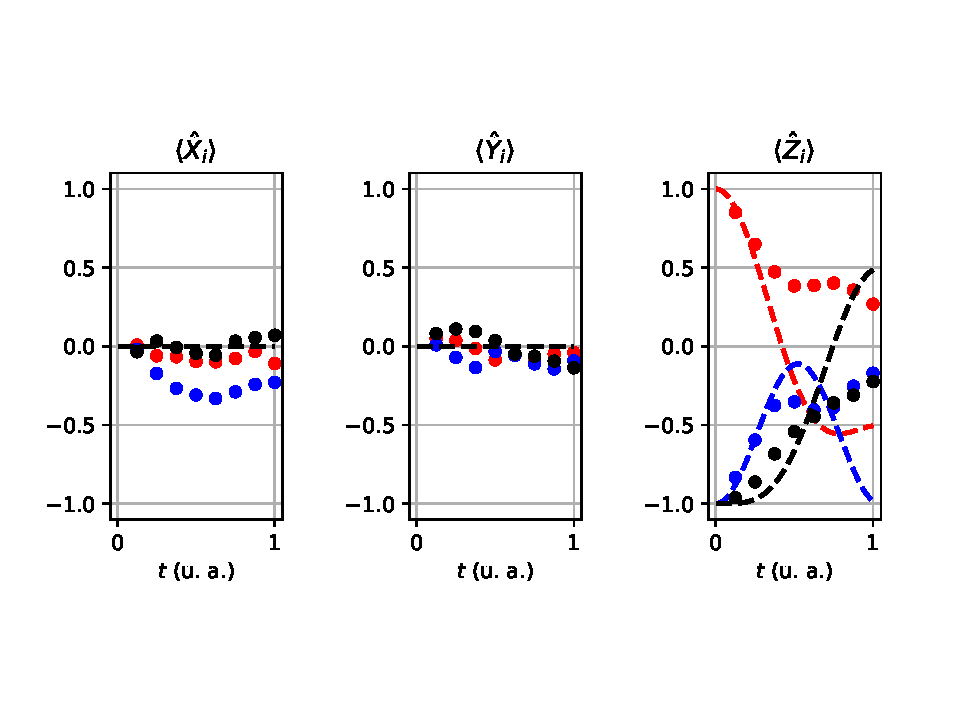
\includegraphics[scale=0.8, trim={0 1.8cm 0 1.8cm}, clip]{BasisEfficientData/basis_efficient_pauli_exps.pdf}
        \caption{Basis efficient expected values}
        \label{fig:PauliBasis}
      \end{subfigure}
      \begin{subfigure}[b]{1.0 \textwidth}
        \centering
        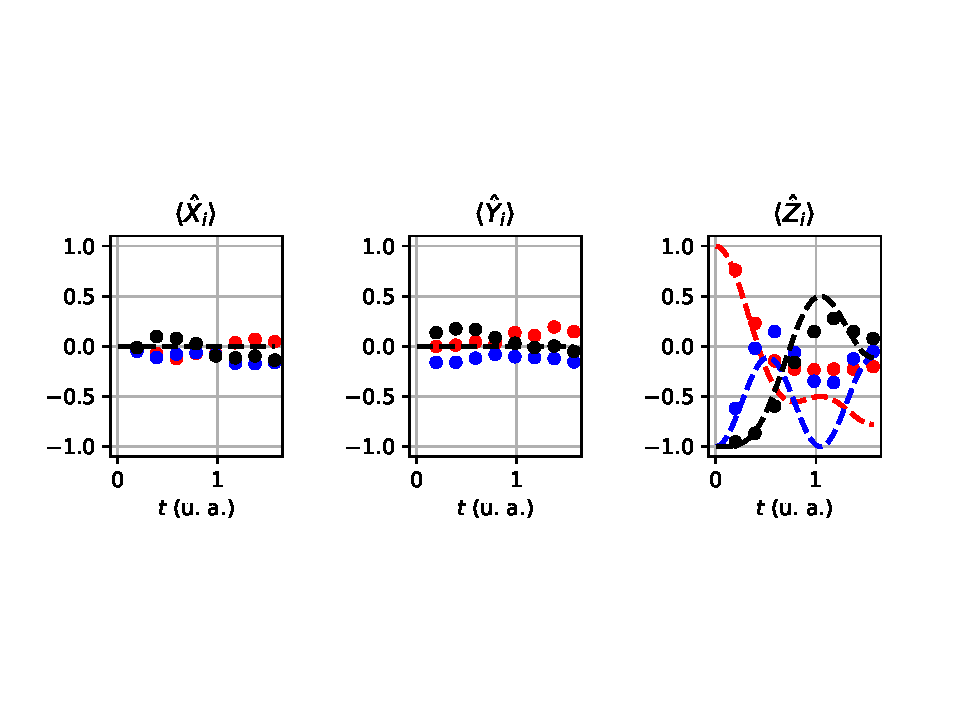
\includegraphics[scale=0.8, trim={0 1.8cm 0 1.8cm}, clip]{PulseEfficientData/pulse_efficient_pauli_exps.pdf}
        \caption{Basis efficient expected values}
        \label{fig:PauliPulse}
      \end{subfigure}
      \caption{Time evolution of single qubit expected values on \textit{ibmq jakarta}. Time units are normalized to $\hbar = 1$. This is denoted bu (u. a.) in the figures.}
      \label{fig:PauliExpectedValues}
    \end{figure}

    \begin{figure}
      \centering
      \begin{subfigure}[b]{0.5 \textwidth}
        \centering
        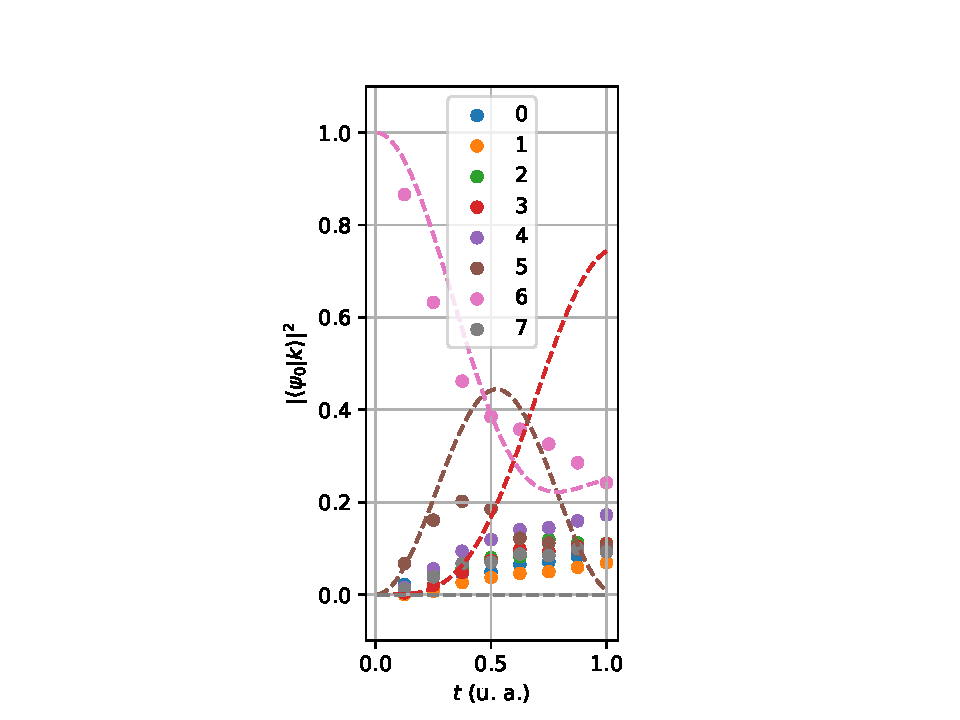
\includegraphics[scale=0.8, trim={2cm 0 2cm 0}, clip]{DirectTranspilationData/direct_pdf_evol.pdf}
        \caption{Direct transpilation pdf.}
        \label{fig:PdfDirectTransp}
      \end{subfigure}%
      \hfill
      \begin{subfigure}[b]{0.5 \textwidth}
        \centering
        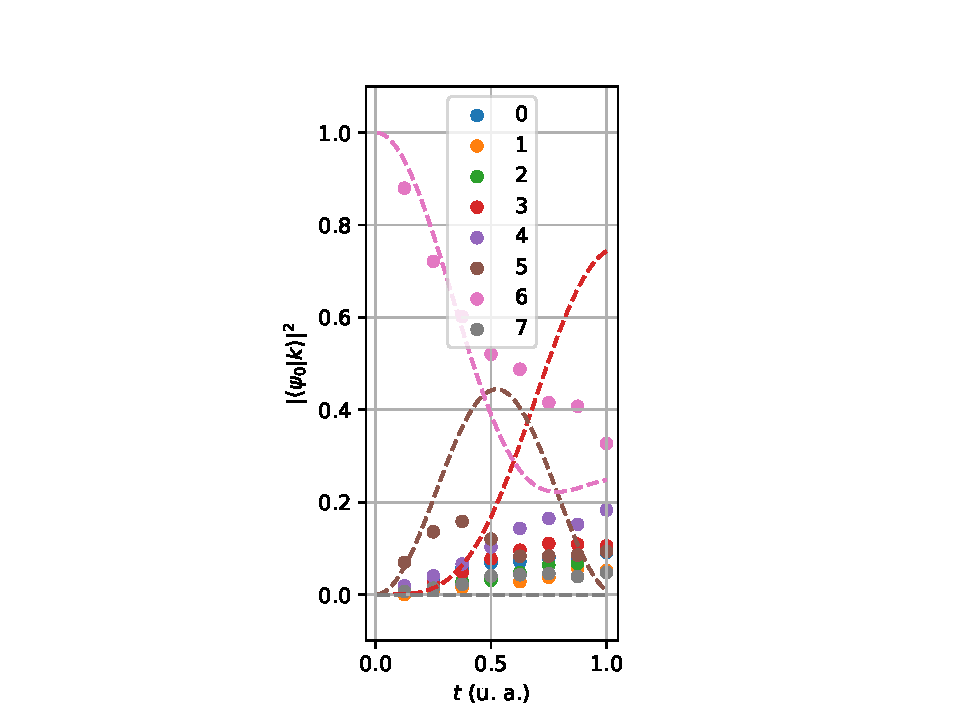
\includegraphics[scale=0.8, trim={2cm 0 2cm 0}, clip]{BasisEfficientData/basis_efficient_pdf_evol.pdf}
        \caption{Basis efficient pdf.}
        \label{fig:PdfBasis}
      \end{subfigure}
      \begin{subfigure}[b]{1.0 \textwidth}
        \centering
        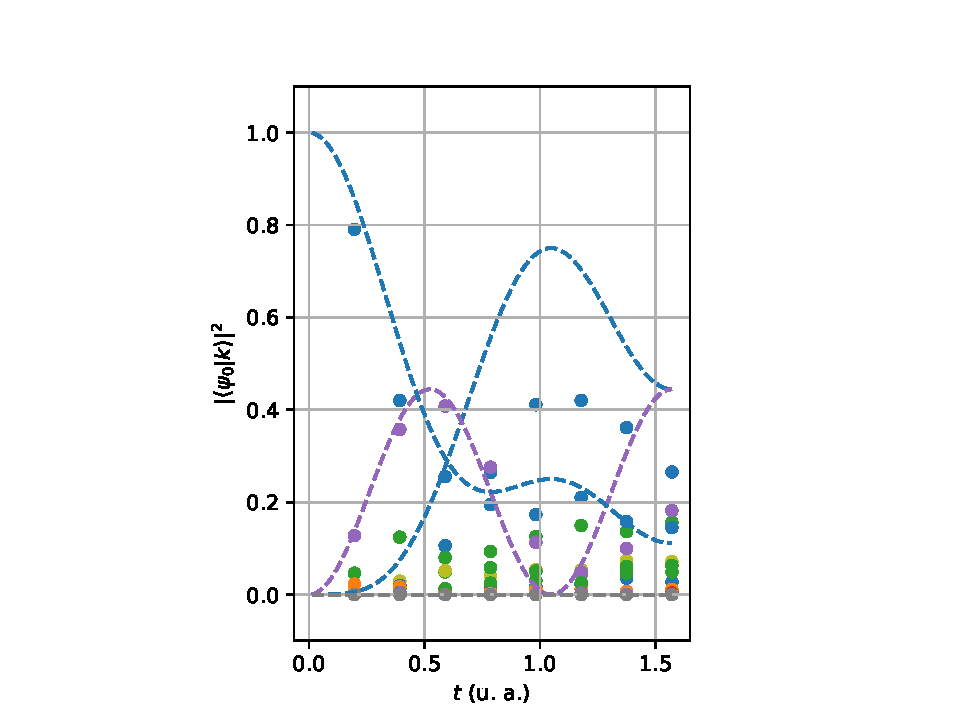
\includegraphics[scale=0.8, trim={1cm 0 1cm 0}, clip]{PulseEfficientData/pulse_efficient_pdf_evol.pdf}
        \caption{Basis efficient pdf.}
        \label{fig:PdfPulse}
      \end{subfigure}
      \caption{Time evolution of benchmark system probability density on \textit{ibmq jakarta}.}
      \label{fig:PdfExpectedValues}
    \end{figure}

    \begin{figure}
      \centering
      \begin{subfigure}[b]{1.0 \textwidth}
        \centering
        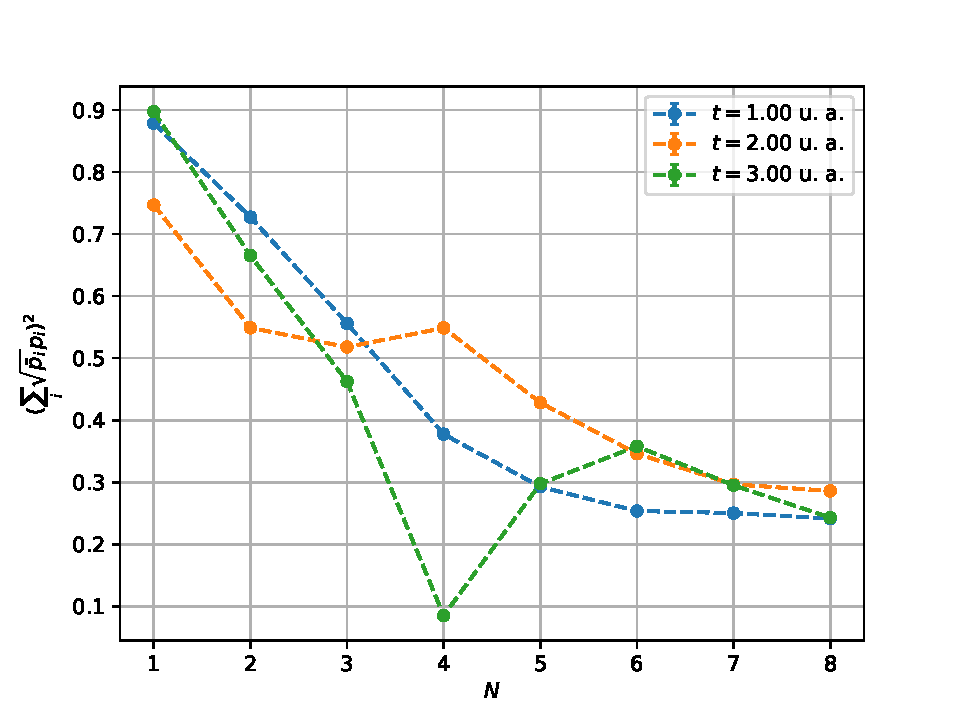
\includegraphics[scale=0.6]{DirectTranspilationData/direct_pdf_fidelity.pdf}
        \caption{Direct transpilation pdf fidelity.}
        \label{fig:PdfDirectTranspFidelity}
      \end{subfigure}
      \begin{subfigure}[b]{1.0 \textwidth}
        \centering
        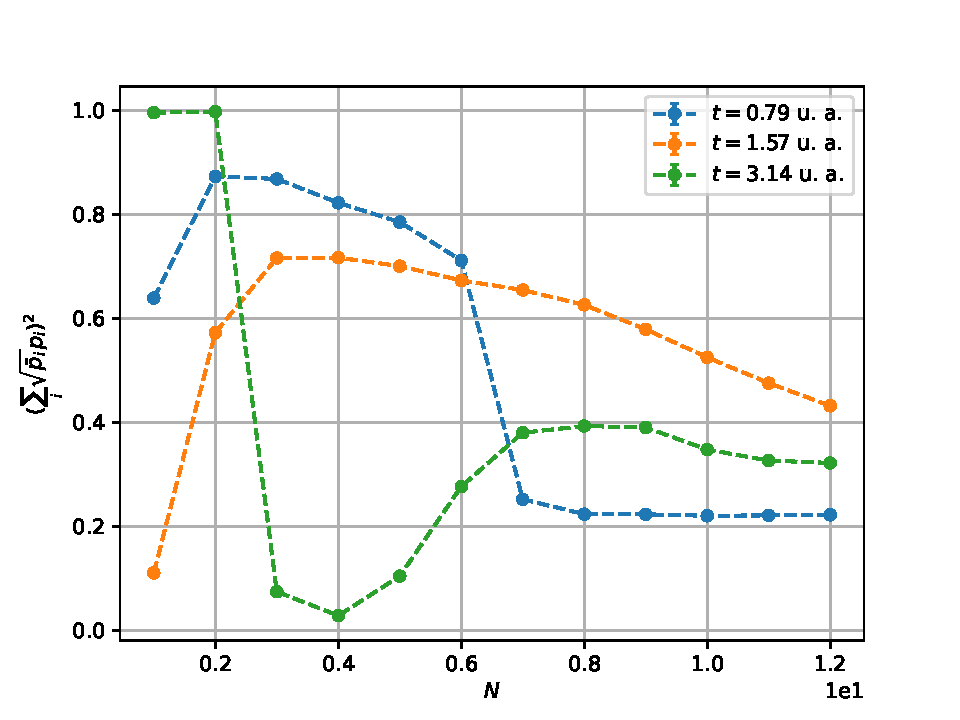
\includegraphics[scale=0.6]{BasisEfficientData/basis_efficient_pdf_fidelity.pdf}
        \caption{Basis efficient pdf fidelity.}
        \label{fig:PdfBasisFidelity}
      \end{subfigure}
      \begin{subfigure}[b]{1.0 \textwidth}
        \centering
        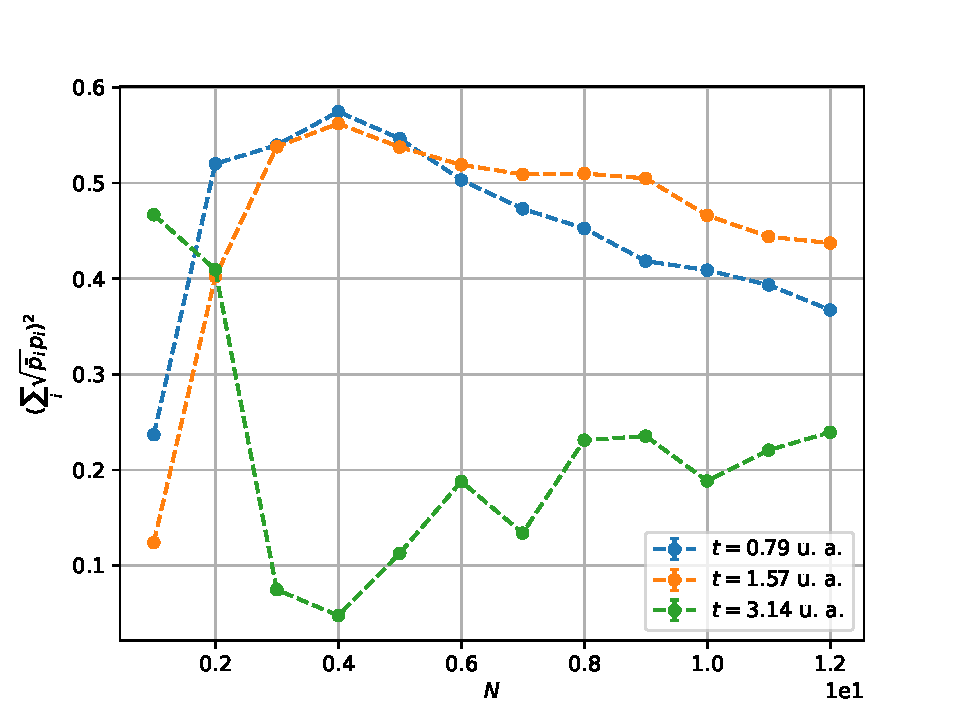
\includegraphics[scale=0.6]{PulseEfficientData/pulse_efficient_pdf_fidelity.pdf}
        \caption{Basis efficient pdf fidelity.}
        \label{fig:PdfPulseFidelity}
      \end{subfigure}
      \caption{Fidelity of benchmark system probability density, w. r. t. ideal state fidelity, when simulated on \textit{ibmq jakarta}.}
      \label{fig:PdfExpectedFidelity}
    \end{figure}

%%%%%%%%%%%%%%%%%%%%%%%%%%%%%%%%%%%%%%%%%%%%%%%%%%%%%%%%%%%%%%%%%%%%%%%%%%%%%%%%
%%%%%%%%%%%%%%%%%%%%%%%%%%%%%%%%%%%%%%%%%%%%%%%%%%%%%%%%%%%%%%%%%%%%%%%%%%%%%%%%
%                    AN APPLICATION TO FERMIONIC SYSTEMS                       %
%%%%%%%%%%%%%%%%%%%%%%%%%%%%%%%%%%%%%%%%%%%%%%%%%%%%%%%%%%%%%%%%%%%%%%%%%%%%%%%%
  \chapter{Variational Quantum Time Evolution}
  \label{chap:vqte}
  \section{Section 1}
  \lipsum[2-4]

\section{Section 2}
  \lipsum[2-4]

\section{Section 3}
  \lipsum[2-4]

\section{Section 4}
  \lipsum[2-4]

%%%%%%%%%%%%%%%%%%%%%%%%%%%%%%%%%%%%%%%%%%%%%%%%%%%%%%%%%%%%%%%%%%%%%%%%%%%%%%%%
%                                BIBLIOGRAPHY                                  %
%%%%%%%%%%%%%%%%%%%%%%%%%%%%%%%%%%%%%%%%%%%%%%%%%%%%%%%%%%%%%%%%%%%%%%%%%%%%%%%%
  \printbibliography
\end{document}
